\documentclass{mcmthesis}
\mcmsetup{CTeX = false,
        tcn = 2010617, problem = C,
        sheet = true, titleinsheet = true, keywordsinsheet = false,
        titlepage = false, abstract = false}
\usepackage{palatino}
\usepackage{lipsum}
\usepackage{enumitem}
\usepackage{subfigure}
\usepackage{multirow}
\usepackage{float}
\usepackage{booktabs}
\usepackage{longtable}
\usepackage{threeparttable}
\usepackage[table,xcdraw]{xcolor}
\title{From data to wealth: textual information extraction and numeric processing}
\date{\today}

\begin{document}

\begin{abstract}


Sunshine Company wants to get advice on the sale strategies on their three products based on data from Amazon.com, especially the time-based patterns. In doing so, we did the following work and provided substantial and detailed conclusions, and in this process we built three main models: 

In the first part, we mined as many measures as we could from the given data sets, mainly using TF-IDF moedel, semantic lexicon and Spectral Co-Clustering algorithm. Based on the mathematically processed and newly extracted measures, we constructed the review helpfulness evaluation model using the comprehensive weighing method of EWM and TOPSIS, and calculate an significant measure 'helpfulness' that indicates how helpful a review is.

In the second part, we focused on the solutions to specific problems:
\begin{itemize}
\item  Aggregate three factors that respectively represent the basic, 'official' and 'unofficial' rating of a review. Then a classified-aggregate regression model is built to find the most informative measures to track. The result shows the 'unofficial' rating matters most, which means measures extracted from consumers not the Amazon.com are vital.

\item  Use the three factors in the previous step to do fitting based on Ordinary Least Squares, and obtain three possible reputation curves. We found the latter two of them can be used to detect trends of reputation.

\item  Detect the inflection points (symbolize the potential success or failure of products) based on MannKenddall method. Then another regression model was built to find the influential measure combinations.
\item  Build a fluctuation correlation analysis model that can examine the sequence and causality between two series. We used it to explore relationship between ratings and review types, and drawed conclusions like high star ratings can incite more positive reviews.
\item  Find out the relationship between ratings and review descriptors on the basis of quantification. And the results vary from descriptors.
\end{itemize}

In the last part, by using TF-IDF together with Co-Clustering, we generated many word clouds that can visually reflect the characteristics of a particular product, which provides specific reference for the improvement of the products.

\end{abstract}

\maketitle

%% Generate the Table of Contents, if it's needed.
\setcounter{tocdepth}{2}
\tableofcontents
\newpage
%% Generate the Memorandum
\memoto{Marketing Director, Sunshine Company }
\memofrom{MCM Team 2010617}
\memosubject{Strategies to win the success of new products}
\memodate{\today}
\begin{memo}[Letter to the Marketing Director]
\noindent Dear Marketing Director,

Textual data and time-based pattern are What's so special about these data sets. Our team put emphasis on these two parts and draw substantial and novel conclusions. Furthermore, our study is able to help you not only with the conclusions, but also with the available models. 

In doing so, our team dug firstly deep into the ratings and reviews of these three products on Amazon using various scientific methods, such as TF-IDF moedel, Dhillons Spectral Co-Clustering algorithm and the comprehensive weighing method of EWM and TOPSIS. 

Then, three models were built during the process to draw useful conclusions from known data: 

 \begin{itemize}
\item the first model evaluates how helpful a review is, which can help you save a lot of energy by selecting the most useful of the many reviews available for analysis after the new products are launched;

\item the second model decides the most informative measures to track for company.

\item the last one can be used to judge the sequence and causality between two sets of numbers, which is helpful for business analysis.

\end{itemize}

In terms of conclusions, we found that:

 \begin{itemize}
\item  The 'unofficial' rating of products is the most informative measures to track. Companies should pay special attention to the quality of customer reviews content, which contributes the most for the sales. To be more specific, to detect the measures such as helpful votes, ratio of helpful, complexity of reviews and so on.
\item  star rating weighted by helpfulness can best detect the trends of reputation.
\item  The measure combinations that can be used to detect the potential success or failure of products are review's two sides attribute (the review contains both negative and positive content, E. G. '...is good, but....'), degree of positive and complexity.
\item  High star ratings can incite more positive reviews. So it's a good idea to find ways to get the high star reviews seen by more customers.
\item  Some descriptors, such as ’great’, is generally strongly associated with rating levels, and the higher the level, the more it appears. However,according to our sentiment measure, although ’great’ appears in 5 star review, it doesn’t necessarily mean this review is positive. But the conclusions vary from different descriptors, as is shown in appendix.
\item We have also extracted features for different products, and visualize them using world clouds. You can intuitively see the keywords of user reviews for each specific product, so as to obtain the potentially important design features that caters to the market. For example, for the hair dryer 423960 ($product\_parent$) with high sales, the feature words include reliable, works well and fancy.
\end{itemize}

Overall product sales on Amazon are increasing year by year, and there are opportunities for companies to bring new products into the store. In our analysis, there are some products where the latter are ahead. We hope our team analysis and results can help you in your online sales strategy and product design. 


%\noinden may cause error
Yours sincerely,

MCM Team 2010617



\end{memo}

\clearpage

\section{Introduction}
\begin{enumerate}
\item Problem Summary

\quad \quad On Amazon, customers can rate and review purchases through the “star ratings” – “reviews” –  “helpfulness rating” mechanism. Sunshine Company wants to  get advice on the sales strategy of its three new products based on existing data, which involves information under Amazon's rating system over the time periods.
\item Our model

\quad \quad The main technical route is as follows:

\begin{figure}[H]
\centering
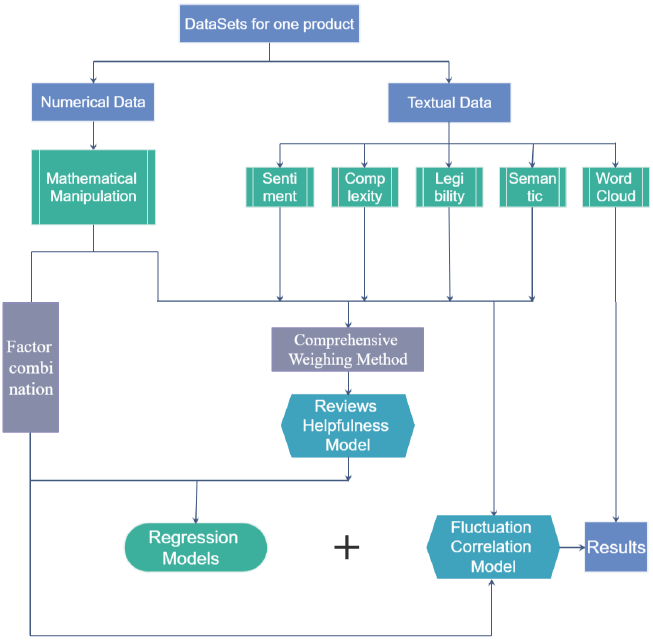
\includegraphics[width=\textwidth]{figures/r.png}
\caption{Technical Route}
\end{figure}
\end{enumerate}

\section{Background}
\quad \quad Analysis  of  online reviews  has an important enlightening effect on  sales  performance and business decision-making[4]. Lots of researches have been conducted in this area, and here are two relevant aspects.
\begin{enumerate}

\item Reviews Helpfulness

\quad \quad Due to the large amount of reviews data, "what factors make a review helpful for potential customers to make purchasing decisions" has become an important research topic. According to a number of studies, consumers tend to judge review helpfulness based on two major features : the extent to which the review familiarizes consumers with the product and the perceived credibility [5]. To be more specific, such as:
 \begin{itemize}
\item  length  : reviews with medium length is considered more helpful
\item  legibility : reviews that are easy to read and understand
\item  sentiment : positive,  neutral, negative or mixed ones
\item  professionalism : a professional consumer's review is more helpful 
\end{itemize}
\item Natural Language Processing

\quad \quad Since reviews are natural language, to extract as much information as possible from them, it is natural to use Natural Language Processing (NLP) technologies.  When apply to the analysis of online reviews, NLP is often used to  do sentiment identification[6,7], semantic analysis[8] and other information retrieval[9,10].
\end{enumerate}

\section{Assumptions}
\begin{itemize}
\item Assuming everyone voted in a fair manner on whether others' reviews are helpful, so the voting results are objective and accurate.
\item Assuming that the reviews written by Customers who were authorized as Amazon Vine Voices are accurate and can be over-weighted.
\item Although someone who bought a product may not review online, there is still a positive correlation between the sales of products and number of reviews, so we can use it as an approximate substitute for sales of particular products.
\end{itemize}

\section{Part \uppercase\expandafter{\romannumeral1}: Mining for the given data sets}
\subsection{Data Preprocessing}

\subsubsection{Missing values processing}
\quad \quad A total of 4 values were found to be missing, two for 'review\_headline' and two for 'review\_body'. 
Considering that the number of missing is small, and there are lots of examples in other reviews have the same contents in 'review\_headline' and 'review\_body' or 'review\_headline' and 'star\_rating' ,for instance, "5" in 'star\_rating' and "Five Stars" in 'review\_headline', we use those two methods to fill missings. The results are shown as follows:
\begin{longtable}{cccc}
    \caption{Fill in missing values}\\
    \toprule
    \makebox[0.3\textwidth][c]{review\_id} &  
    \makebox[0.1\textwidth][c]{star\_rating} &
    \makebox[0.25\textwidth][c]{review\_headline} &  
    \makebox[0.25\textwidth][c]{review\_body} \\
    \midrule
    \endhead
    \bottomrule
    \endfoot
    R74VTHE48J4IQ & 3 & Smaller & \underline{Smaller}  \\
    R3BVF5UJ5TMXHK & 5 & Five Stars & \underline{Five Stars}  \\
    R2TW4FSXQ60M75 & 5 & \underline{Five Stars} & Used once ...  \\
    R24Y12M6JKTTQM & 4 & \underline{Four Stars} & It is very nice ...  \\
    \end{longtable}
\subsubsection{Duplicate values processing}
\quad \quad We found 4 and 12 duplicate values in each of the two datasets, microwave ovens and baby pacifiers.
While it's reasonable for parents to buy a pacifier product several times at the same date and write same reviews, it seems that the duplicated reviews of microwave oven, written by a person for 4 times at a single day, are just repeated complaints about his awful experience. Also given that all the duplicated pacifier reviews were purchase-verified which were not for ovens', we keep all the pacifier reviews but only one for those 4 duplicated microwave oven reviews.
\subsubsection{Generate new features}
\quad \quad We combine some ratio-like features. For example, we divide the $total\_votes$ by $helpful\_votes$ to get $helpful\_ratio$. 
\subsubsection{Data Normalization}
\qquad Normalization can provide an approach for comparison of different numerical features and reflect the combined results of different factors.\par
We use min-max normalization, doing linear transformation of the raw data, mapping data set $x=\{x_1, x_2, \ldots, x_n\}$ into $[0, 1]$. The normalized value is
\begin{equation}
    x' = \frac{x-x_{min}}{x_{max}-x_{min}},
\end{equation}

\subsection{Review Information Extraction}
\subsubsection{Extract structured word vector}
\quad \quad Algorithms often cannot directly process text data so we need to extract some features out of the texts and convert them into numeric features.\par
We focus on our attention on using TF-IDF model to remove stop words and extract key features hiden in the 'review\_body'. In a given document, term frequency (TF) refers to how often a given term appears in the document. If a word appears very frequently in a particular document and very low in other documents, then the word is likely to be a word unique to the document and can describe the document well. Word $d_{i}$'s frequency $TF_{ij}$ in document $D_j$ is:
\begin{equation}
    TF_{ij}=\frac{n_{ij}}{n_{dj}}=\frac{n_{ij}}{\sum_k {n_{kj}}}
\end{equation}\par

with $n_{ij}$ is the number of occurrences of the keyword  $d_i$ in the document $D_j$, $n_{dj}$ is the total number of words in the document $D_j$.
And inverse document frequency is defined as below:
\begin{equation}
    IDF_i=\log{\frac{N}{d}}=\log{\frac{N}{\{j:d_i \in D_j\}}}
\end{equation}\par

with $N$ is the total number of documents in the data set, and $d$ is the number of documents containing the keyword $d_i$.
And finally we get TF-IDF:
\begin{equation}
    TF-IDF_i=TF_{ij} \cdot IDF_i
\end{equation}
\subsubsection{Sentiment Extraction}
\quad \quad The TF-IDF vectorized posts form a word frequency matrix, which is then biclustered using Dhillon’s Spectral Co-Clustering algorithm. 

Clusters rows and columns of an array $X$ to solve the relaxed normalized cut of the bipartite graph created from $X$ as follows: the edge between row vertex $i$ and column vertex $j$ has weight $X[i, j]$.

For a few of the best biclusters, its most important words get extracted. Then look each word  up in a senti-dictionary, called $vader\_lexicon$, and compute its tendency to three attitude levels: $positive$, $negtive$ and $neutral$. We calculate three scores for each review accordiing to those three attitude level. Then we do normalization to make three scores sum up to 1 and generate the sentiment vector.
\subsubsection{Legibility Extraction}
\quad \quad A large number of studies have shown that lexical and syntactic difficulties have a high predictive power for text legibility. For General Purposes, formulas containing these two variables can make fairly accurate and direct predictions of text legibility[11]. 
In this paper, we make use of the vocabulary angle, based on the study of vocabulary in Brown Corpus to compile the common vocabulary list, and according to the coverage of words in these lists to the text corpus, we can determine the legibility of the text. And from that, we've got the new measure $understandable$ which can range from 0 to 1.
\subsubsection{Complexity Extraction}
\quad \quad Once the $understandable$ feature is done, we can easily define a new feature called 'complexity'. As reviews with strong legibility can convey their thoughts and feelings to other people immediately, a review with strong complexity may introduce more detailed informations. We'd like to find out whether detailed reviews will affect the sales of the product. The reviews' $complexity$ can be difined as follw:
\begin{equation}
    complexity = e^{-understandable}, \quad understandable \in [0,1]
\end{equation}
with $complexity$ also range from 0 to 1 and is negatively related to $understandable$.

\subsection{Evaluation Model for Reviews Helpfulness}
\quad \quad In order to make the best use of the textual information of reviews, it is necessary to evaluate their helpfulness. On the basis of combing the previous conclusions in this field, we put forward an evaluation system model which is suitable for the existing data sets. On the basis of extracting the effective patterns and measures( hereinafter together referred to as the indexes ), the comprehensive weighting method of Entropy-weight and TOPSIS is applied, and we successfully obtained the helpfulness degree of each comments.

\subsubsection{Establishment of Index System}
\quad \quad As for indexes, $helpful\_votes$ and $helpful\_ratio$ reflect two different mindsets among consumers: some are more focused on the quantity of reviews, while others prefer quality; vine can be used to determine whether a reviewer is "professional" and make whose review objective and clear. The indicators we have selected are shown in the table below.
\begin{table}[H]
    \centering
    \caption{Indexes for Review Helpfulness Evaluation}
    \begin{threeparttable}
    \resizebox{.95\textwidth}{!}{
    \begin{tabular}{cccc}
    \toprule
    Index     & Type         & Value         & $P/N^*$ \\
    \midrule
    helpful\_votes     & Quantitative & Non-negtive Integer      & P   \\
    helpful\_ration    & Quantitative & Decimal between 0$\sim$1 & P   \\
    understandable     & Quantitative & Decimal between 0$\sim$1 & P   \\
    complexity         & Quantitative & Decimal between 0$\sim$1 & N   \\
    vine               & Qualitative  & Boolean Y/N              & P   \\
    verified\_purchase & Qualitative  & Boolean y/n              & P   \\
    sides              & Qualitative  & One-sided or Two-sided   & /   \\
    \bottomrule
    \end{tabular}}
    \begin{tablenotes}
    \footnotesize
    \item[*] $P/N$ illustrates whether the effect on helpfulness is positive or negative
    \end{tablenotes}
    \end{threeparttable}
\end{table}

We also work with reviews' $sides$ when measuring review contents. People may often consider two-sided reviews to be more helpful than one-sided ones when the reviewers are experts[12].
$verified\_purchase$ is another important index which confirms the purchase. When a review is understandable, which means it doesn't use many obscure words or grammars. Higher readability makes the review become more helpful while complexity may introduce more details about the product which should be also taken into considerations[13].

\subsubsection{Comprehensive Weighting Methodology}
\quad \quad Now suppose there are $p$ reviews, which poses the alternative set; $n$ evaluation indexes, which poses the criteria set; then we can get the decision matrix $X=[x_{ij}]_{p\times n}$.

To obtain more reasonable weighting results, we adopted the combination of 'Entropy-weight' method and 'TOPSIS' method, whose principles are as follows:

\begin{enumerate}[leftmargin=*,fullwidth,itemindent=2em,label=(\arabic*)]

\item{Entropy Weight Method}

\quad \quad When applied to the entropy weight method, the higher the entropy value, the less effective information the index carries, and the more chaotic the system.
Assuming that the data have been non-negative processed, the entropy of the $j$th evaluation index can be calculated:
\begin{equation}
    H_j=-{(\ln{n})}^{-1} \sum_{j=1}^p {q_{ij}}{\ln{q_{ij}}}
\end{equation}
\quad \quad with $q_{ij}=x_{ij}/\sum_{i=1}^p {x_{ij}}$ represents the proportion of the $i$th review in the $j$th index. Further, the entropy weight of the $j$th criterion can be calculated, and then the entropy weight method score of each review can be calculated as below:
\begin{equation}
    W_j = \frac{1-H_j}{n-\sum_{j=1}^n {H_j}}
\end{equation}

\item{TOPSIS Method}

\quad \quad TOPSIS is another method based on the distance between the chosen alternative and the ideal solution. Here the optimal score of a certain attribute of review is the ideal solution of this attribute, while the negative ideal solution is the opposite, indicating the worst score of a certain attribute. We calculate the distance from the $i$th review to the positive ideal solution negative ideal solution by following formulas:

\begin{equation}
d_{1j}=\sqrt{\sum_{j=1}^n {(x_{ij}-a_j)}^2},\quad d_{2j}=\sqrt{\sum_{j=1}^n {(x_{ij}-b_j)}^2}
\end{equation}\par

\quad \quad Finally, we calculate the TOPSIS score of the $i$th review by those two distances above:

\begin{equation}
    y_i = \frac{d_{2i}}{d_{1i}+d_{2i}}
\end{equation}

\end{enumerate}

\subsubsection{Calculation and Results}
\quad \quad We calculate the comprehensive weighting method based on a performance matrix composed of four numerical indexes, namely   $helpful\_votes$, $helpful\_ratio$, $understandable$ and $complexity$. Since the four indexes were given by lots of consumers, which means it's "public and unofficial", unlike $vine$ and $verified\_purchase$, which are given directly by Amazon.com. So we call the results of this stage "Unofficial Helpfulness". Due to space constraints, table 2 only shows 7 reviews out of 32021. All the results are shown in appendix. 

\begin{longtable}{ccccc}
\caption{Resluts of Helpfulness for Each Review}\\
\toprule
\makebox[0.2\textwidth][c]{review\_id} &  
\makebox[0.15\textwidth][c]{Entropy-Rank} &
\makebox[0.15\textwidth][c]{Entropy-Score} & 
\makebox[0.15\textwidth][c]{TOPSIS-Rank} &  
\makebox[0.15\textwidth][c]{TOPSIS-Score } \\
\midrule
\endhead
\bottomrule
\endfoot
R35BHQJHXXJD59 & 16705.5     & 0.028909     & 16729.5 & 0.001014 \\
R230LCPQDOFJJZ & 24633.5     & 0.027926     & 24638.5 & 0.000733 \\
R21NN9ONVZITI0 & 29482       & 0.001702     & 29482   & 0.000312 \\
R18NK8BQ5LPMZZ & 24633.5     & 0.027926     & 24638.5 & 0.000733 \\
R2NEOR5Y0P7U8V & 17808.5     & 0.027681     & 17828.5 & 0.000983 \\
$\cdots$       & $\cdots$    &  $\cdots$    & $\cdots$& $\cdots$  \\
R3N0F2FKJOMGKK & 2764.5      & 0.354135     & 1776.5  & 0.015989 \\
R2WDYCZI91LL6K & 27390       & 0.021149     & 27391   & 0.000558 \\
\end{longtable}

Though the scores of Entropy-weight method and TOPSIS method are different in the overall size, but from the ranking point of view, the two results are correspondent which shows the comprehensive method of weight is very effective.

The second step is to apply Boolean indexes to score. When both conditions $vine$ is 'Y' and $sides$ is 'two-sided' are met, the score is rewarded; when $verified\_purchase$ is 'n', the score is reduced. The results obtained after this stage are comprehensive helpfulness:
\begin{equation}
    \begin{aligned}
    Comprehensive Helpfulness &= Official Helpfulness \\
    &+ Unofficial Helpfulness
\end{aligned}
\end{equation}\par

Now we have the helpfulness value for each review, which provides an important reference for exploring the role of review in business strategy.

\section{Part \uppercase\expandafter{\romannumeral2}: Analysis and solution of specific problems}
\subsection{Most Informative Measures to Track}
\quad \quad To find out the most informative measures, we construct a classified-aggregate regression model of three factors, constructs their regression relationship with sales.
The dependent variable here is a $products' sales$, because it's the final transformation results and the most concern of business operators.

Among various extraction ways we have, $star\_rating$ is the most basic and intuitive feature to show a consumer's feeling, which is also the first layer of Amazon's mechanism. We can generate a scatter plot between the sales and  $mean\_star\_rating$ of each hair dryer, aggregated by $product\_parent$. However, the plot turn out to be meaningless as all the points gathered together around a high $star\_rating$ while sales are very different. Therefore, review-based measures are essential and needed to be added.

\begin{figure}[H]
\centering
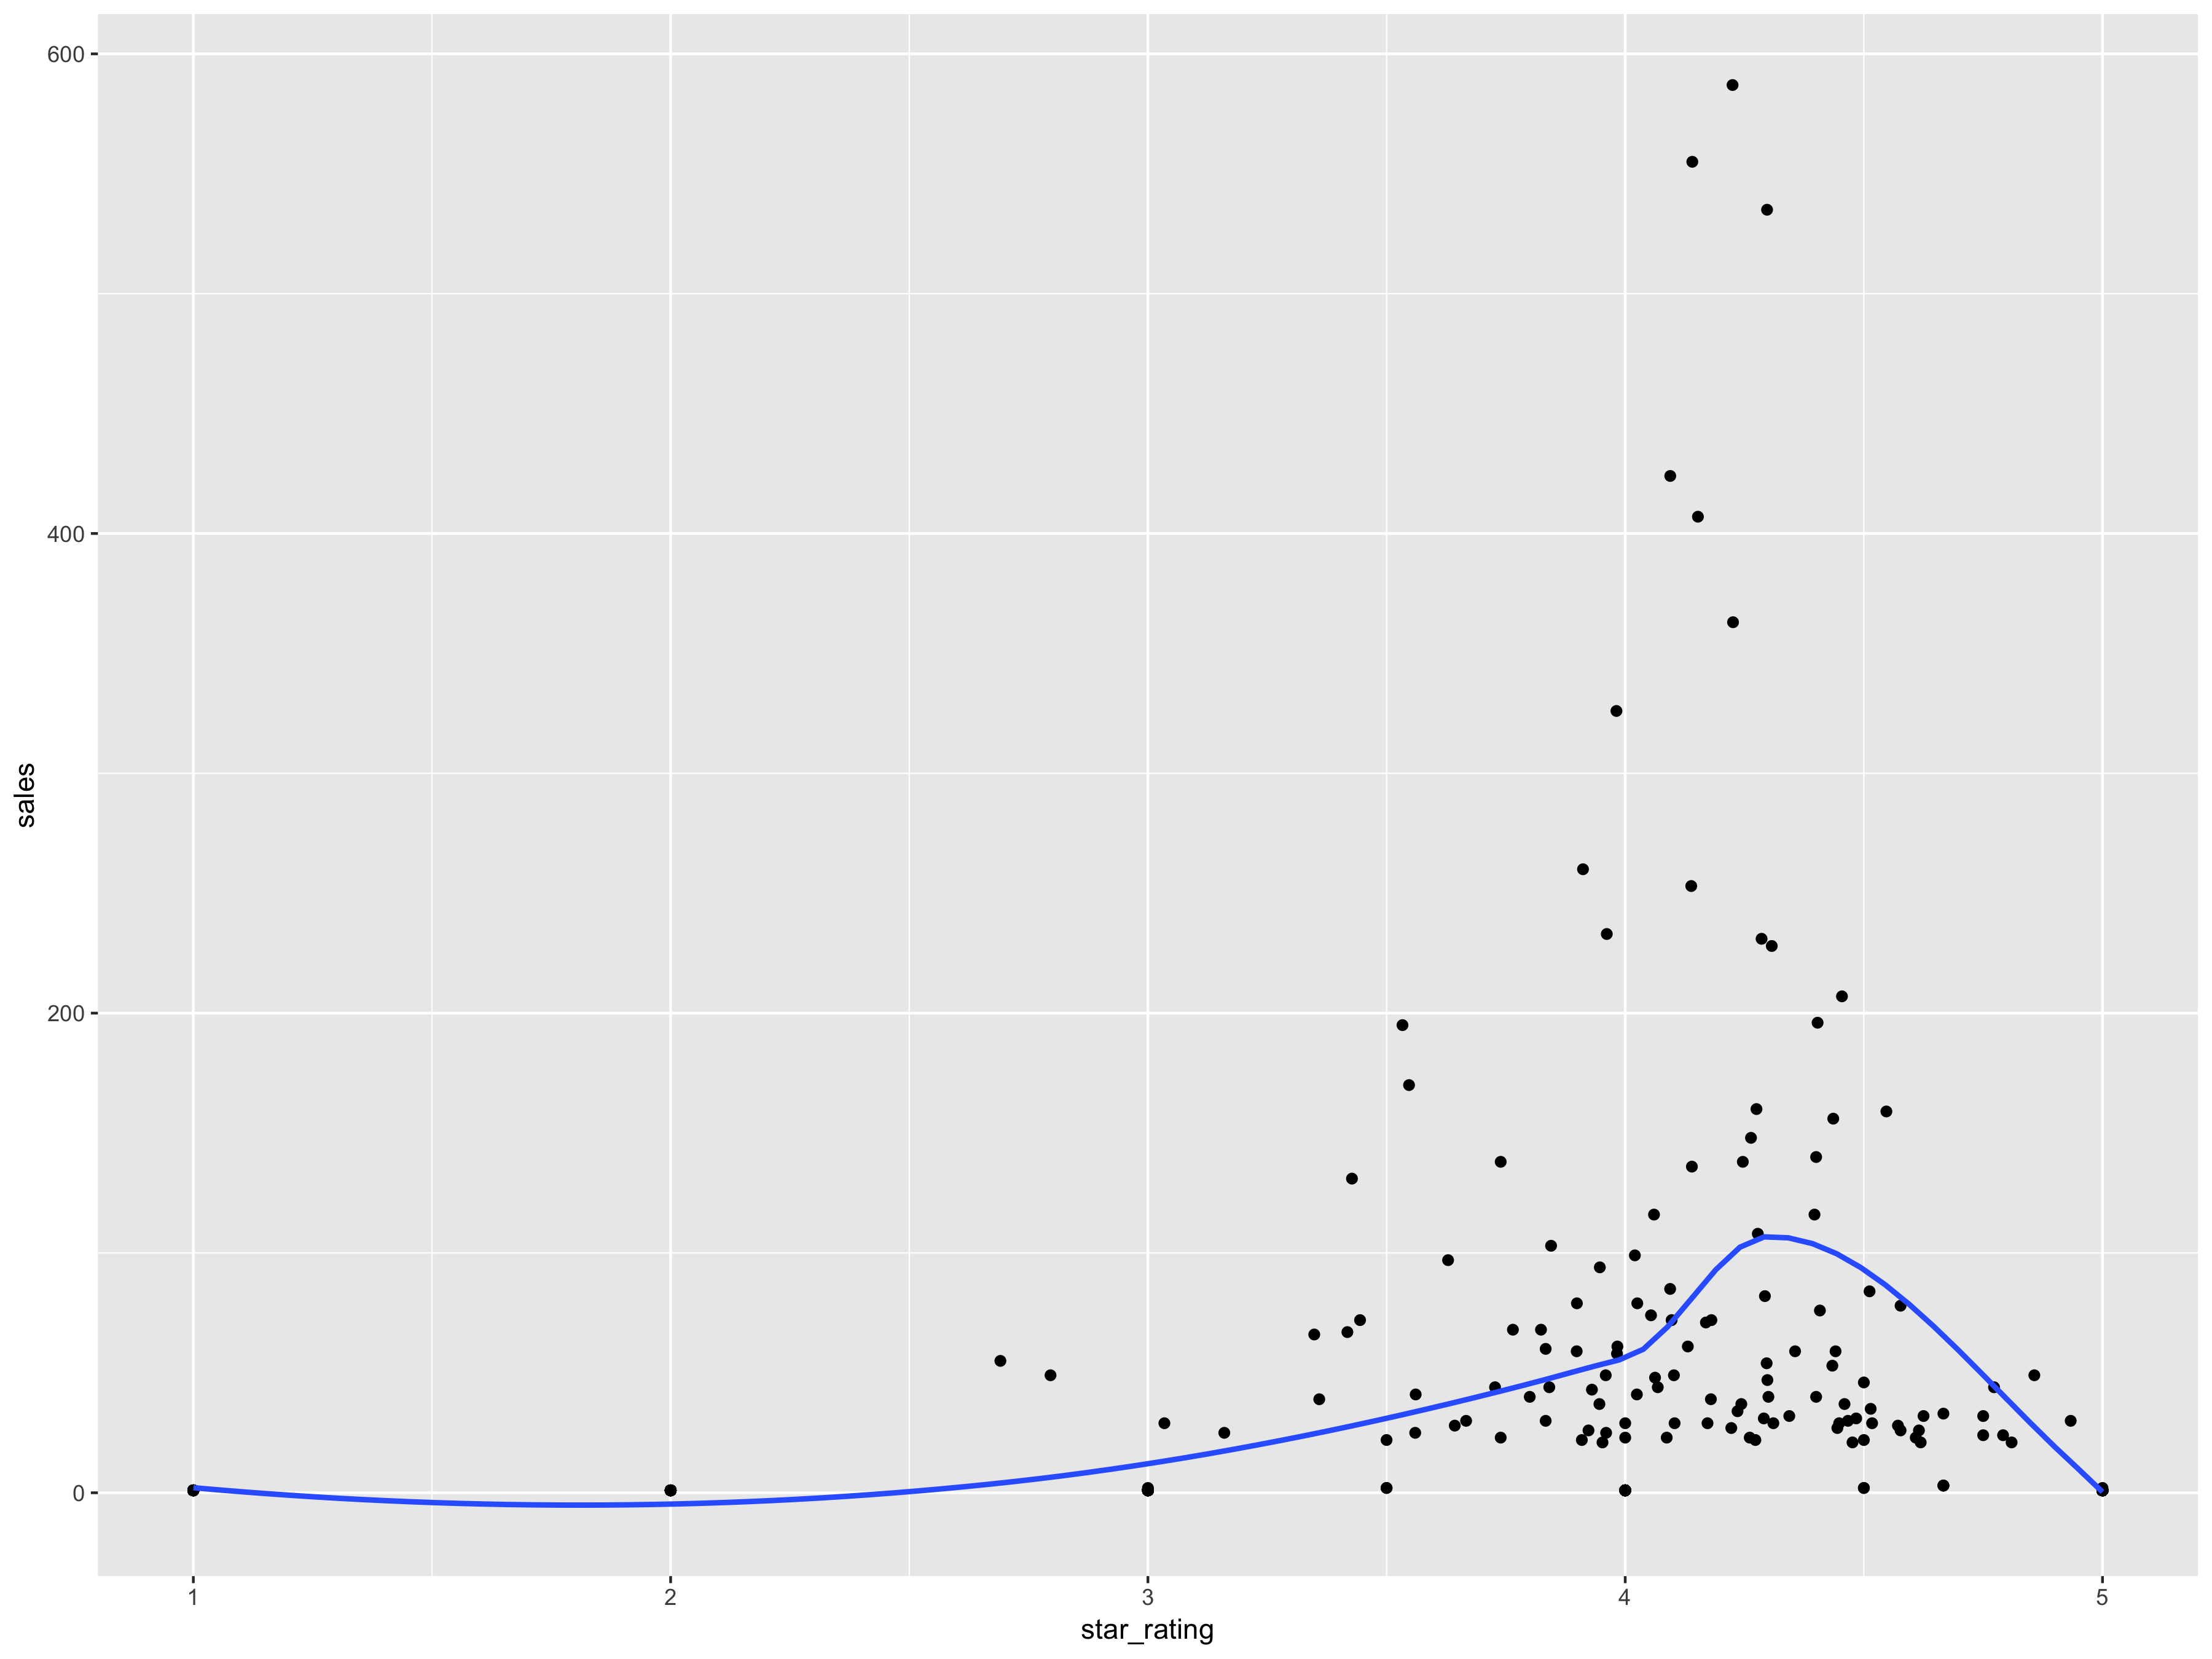
\includegraphics[width=.8\textwidth,height=5.8cm]{figures/2.png}
\caption{mean\_star\_rating for each dryer}
\end{figure}

When considering review-based measures, similar to part 4.3, we classify them into two types, Official and Unofficial. Actually, the measures are used to calculate the helpfulness of reviews, so we aggregate these measures by type and amplify the basic $ star\_rating$:
\begin{itemize}
    \item $x_{1}$ : $ star\_rating=r$
    \item $x_{2}$ : $ rate\_exp\_num = r \times e^{vine+verified\_purchase} $
    \item $x_{3}$ : $ rate\_exp\_txt = r \times e^{helpfulness+two\_sides} $
\end{itemize}

 Now we can generate dryers' sales scatter plots respectively based on $rate\_exp\_num$ and $rate\_exp\_txt$, which are significantly better than before:
 
 \begin{figure}[H] 
  \centering 
  \subfigure[rate\_exp\_num]{ 
    %\label{fig:subfig:a} %% label for first subfigure 
    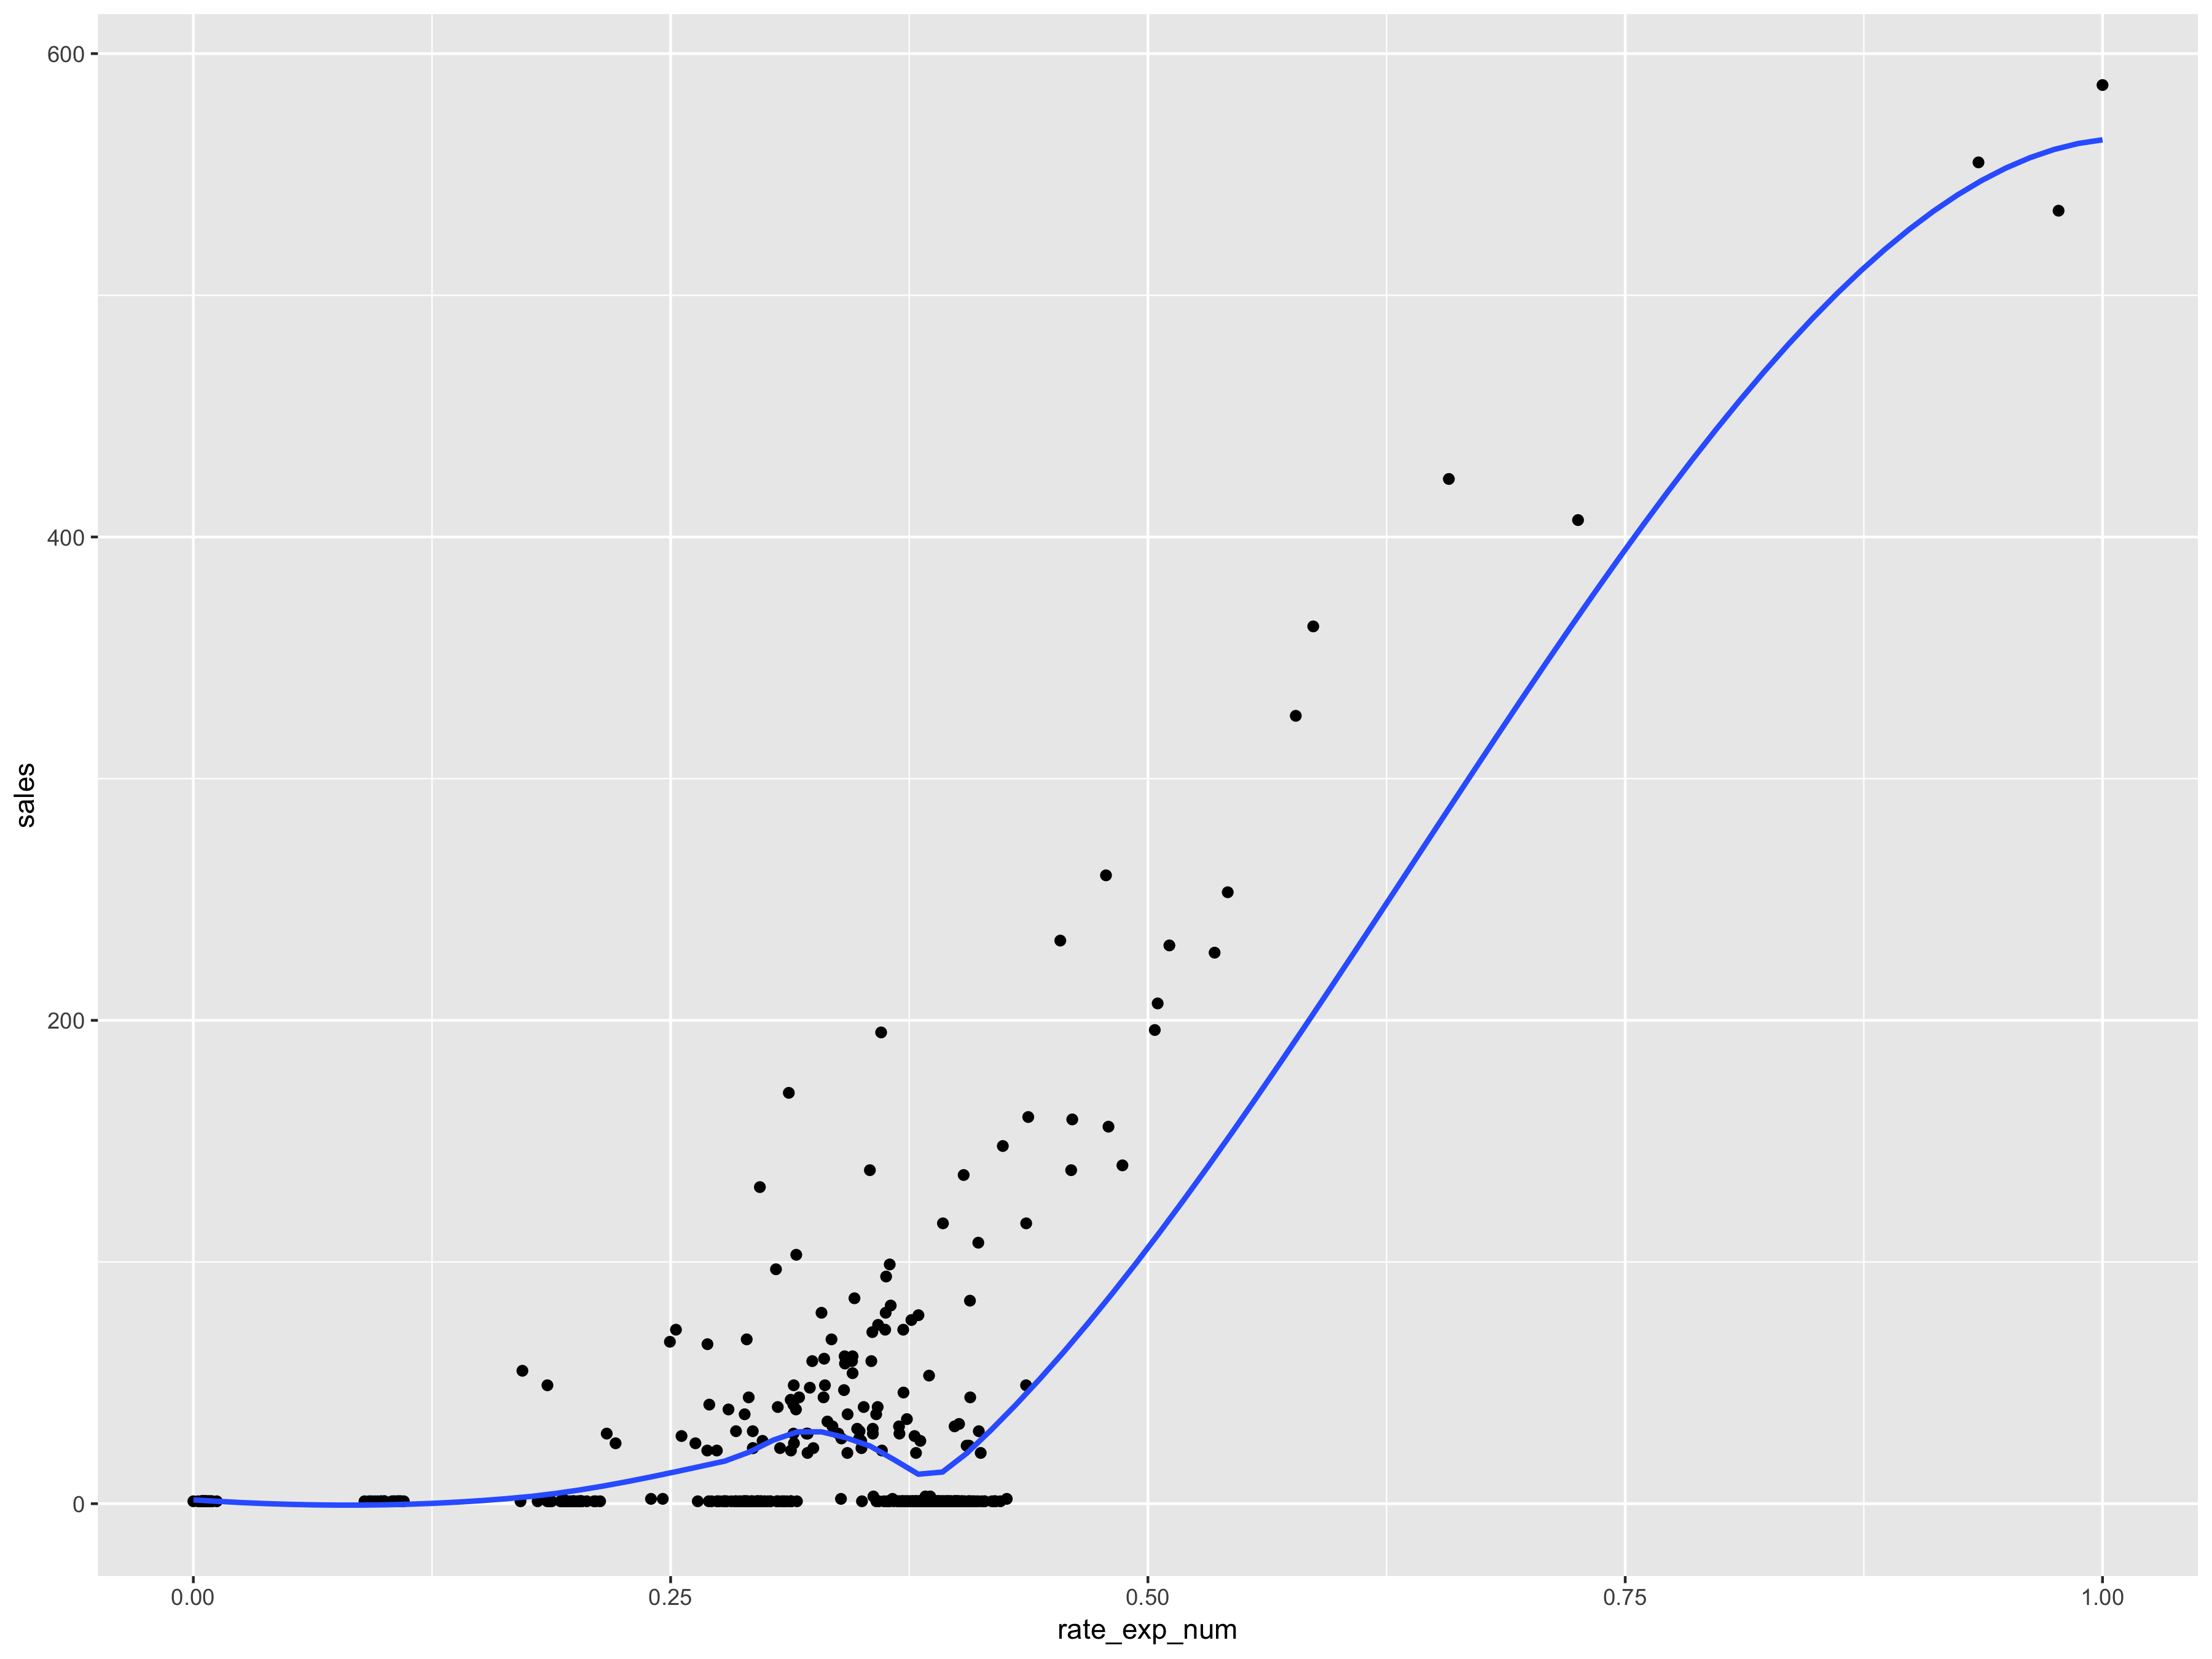
\includegraphics[width=.48\textwidth]{./3.png} 
  } 
  \subfigure[rate\_exp\_txt]{ 
    %\label{fig:subfig:b} %% label for second subfigure 
    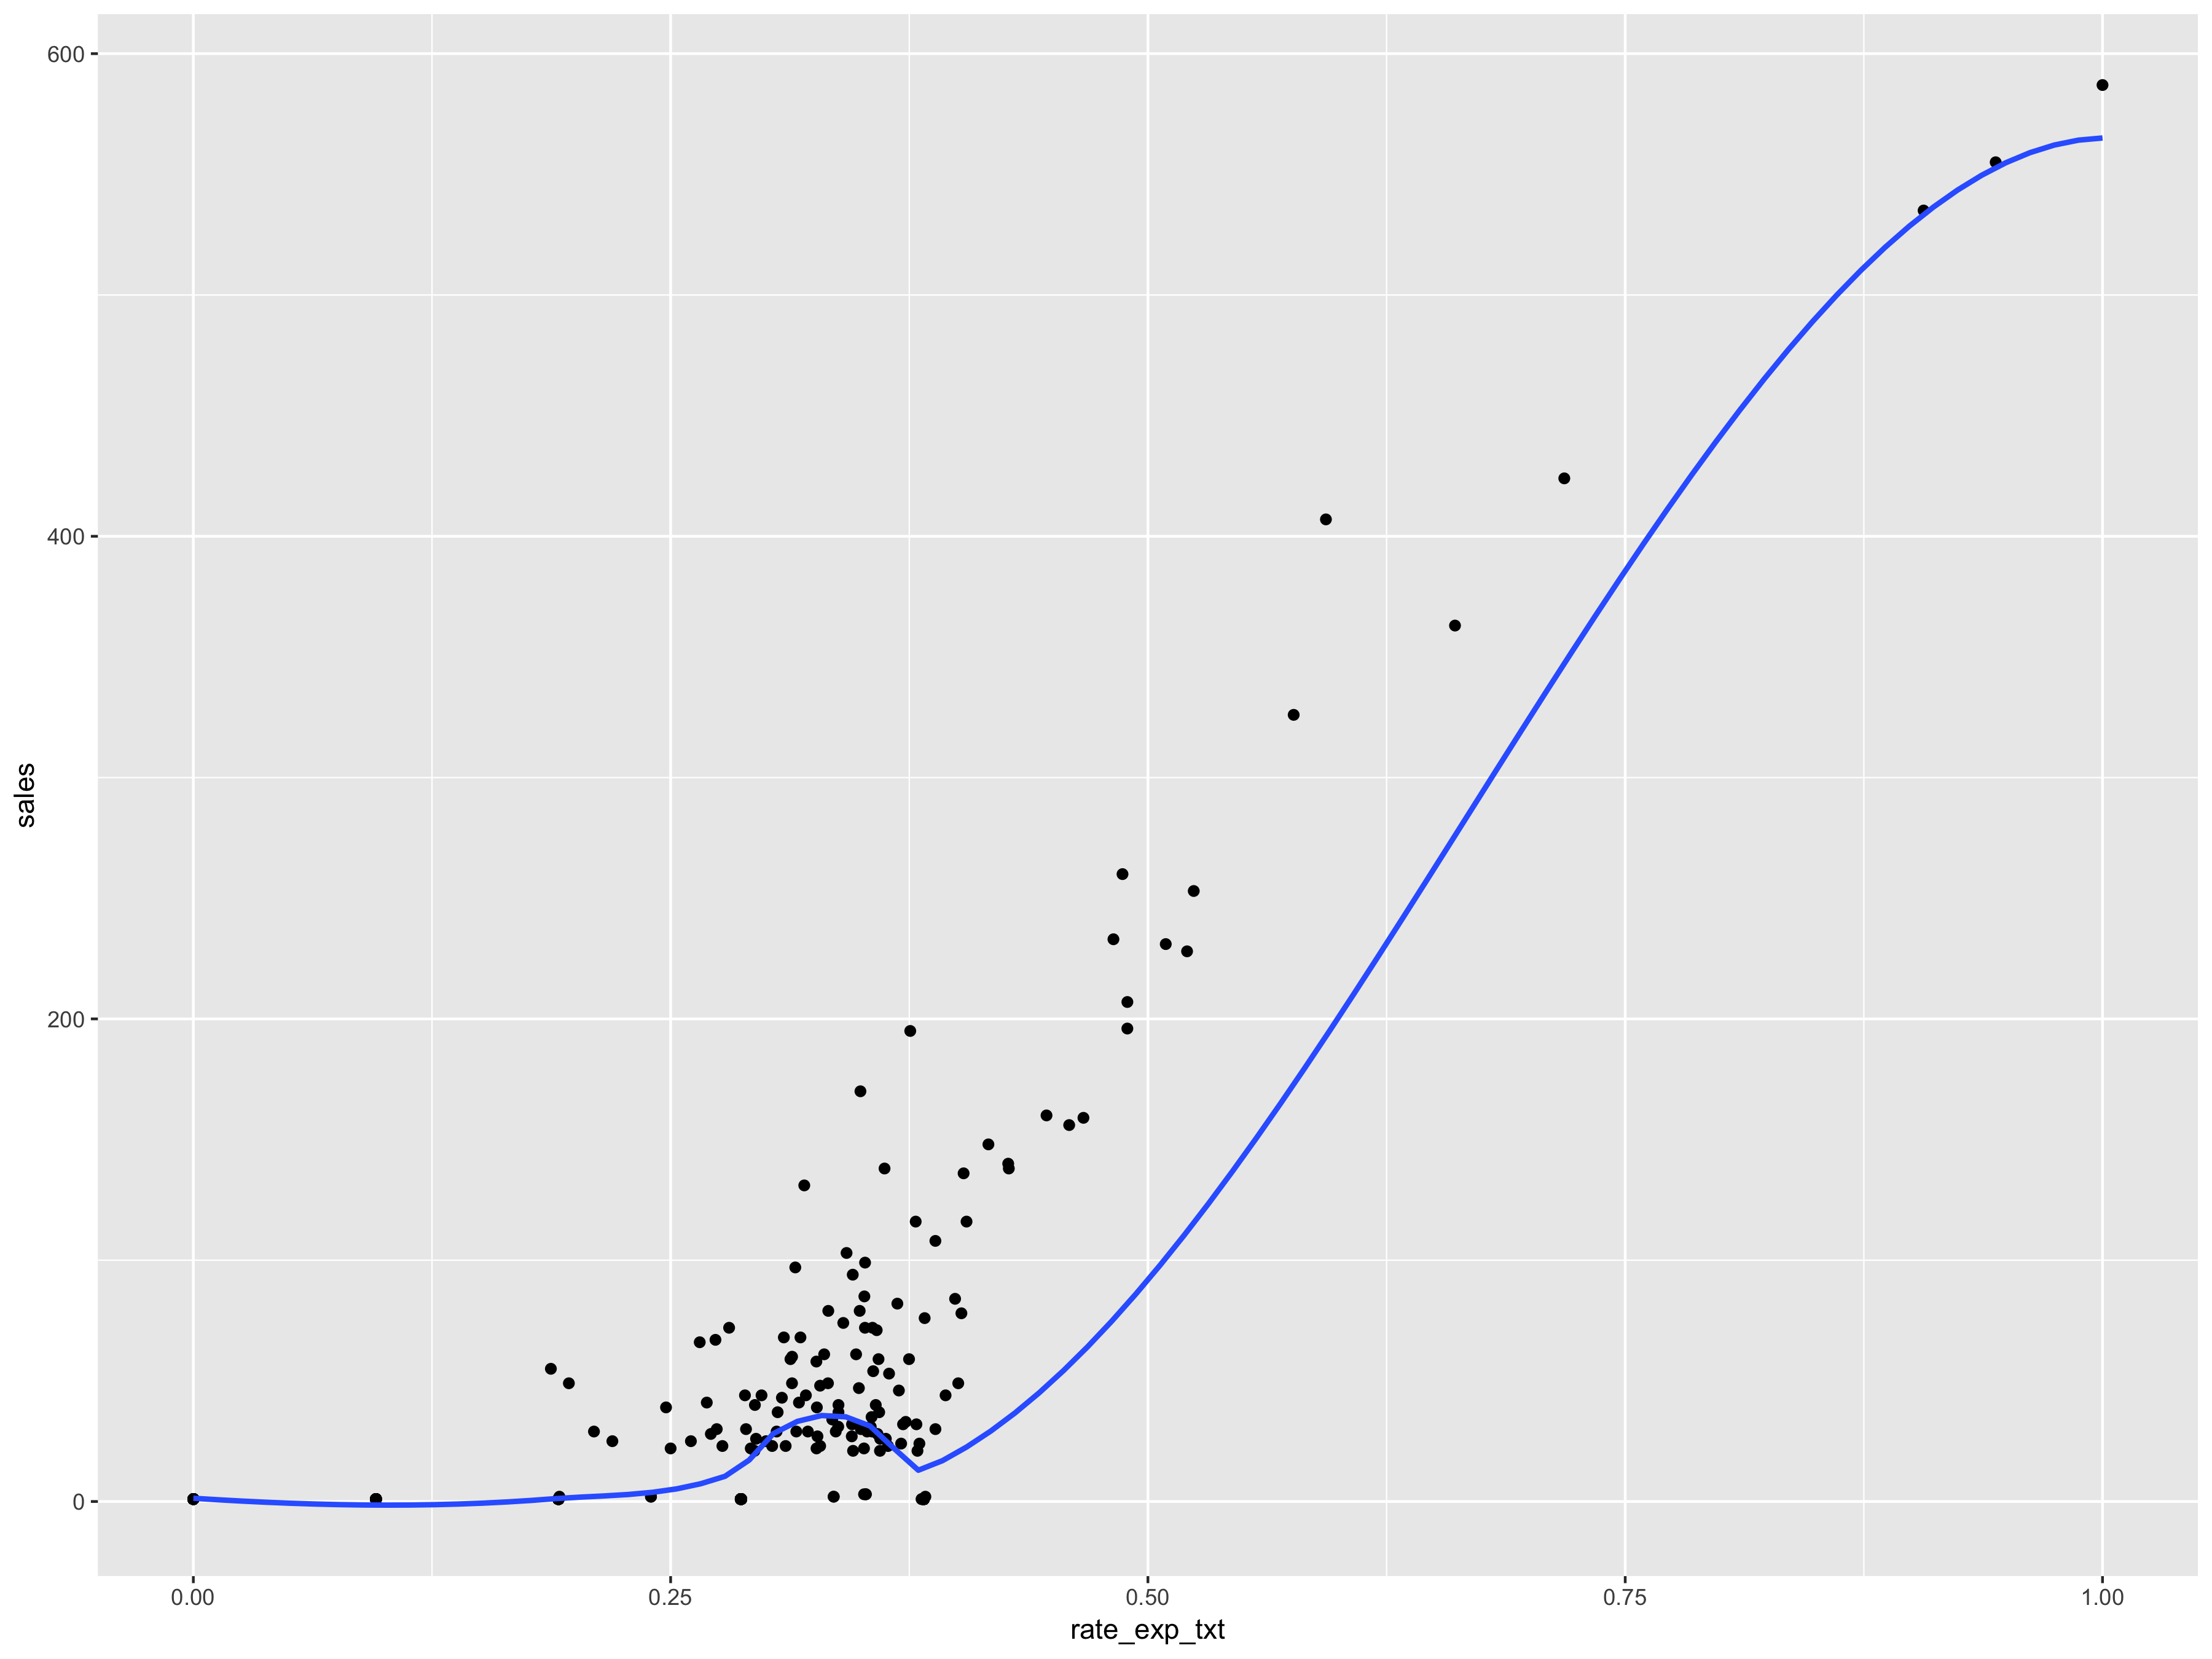
\includegraphics[width=.48\textwidth]{./4.png} 
  } 
  \caption{Frames of the house and hotel data sets} 
  %\label{fig:subfig} %% label for entire figure 
\end{figure}
 
Then we use linear regression model to fit products' sales and above three rating meatures. The results of three products are respectively shown in the table, which summarizes the importances of each measure variables:

\begin{longtable}{cccc}
\caption{Importance given by Regression Model}\\
\toprule
\makebox[0.25\textwidth][c]{measure variables} &  
\makebox[0.2\textwidth][c]{hair\_dryer} &
\makebox[0.2\textwidth][c]{microwave} & 
\makebox[0.2\textwidth][c]{pacifier} \\
\midrule
\endhead
\bottomrule
\endfoot
rate\_exp\_txt & 0.7782913   & 0.4796037 & 0.5996864 \\
rate\_exp\_num & 0.1499111   & 0.4028003 & 0.3184868 \\
star\_rating   & 0.0717975   & 0.1175959 & 0.0818266 \\
\end{longtable}

As is shown in the table, for all of the three products, the independent variable that has the greatest impact on sales is $rate\_exp\_txt$, which indicates that unofficial feelings about reviews have greater importance. Therefore, companies should pay special attention to the qualify of customer reviews content, which contributes the most for the sales. To be more specific, such as reviews' $helpful\_votes$, $helpful\_ratio$, $complexity$ and so on.

\subsection{Measures that Suggests Reputation Trends}
\quad \quad Considering where they came from, all of the above three variables $rate\_exp\_txt$, $rate\_exp\_num$ and $star\_rating$ can represent the reputation. The $star\_rating$ is the basic and intuitive symbol of reputation, while the other two are the scale-up of it based on different priorities. 

In order to explore the trend of reputation change of each product, we fit the measures that can represent reputation in a chronological order, with specific steps as follows:

\begin{itemize}
\item  Step 1 : Time aggregation

\quad \quad Since the amount of data per day is too large, we first aggregate the data on a monthly basis, and the values of the three reputation variables are averaged. After aggregation, there are nine($3 \times 3$) reputation measures in time series.

\item  Step 2 : Draw the scatter plots

\quad \quad According to the distribution of scattered points, the approximate and suitable curve type can be selected. We draw the nine scatter plots in this step. For example, the scatter plot of star\_rating for hair dryer:

\begin{figure}[H]
\centering
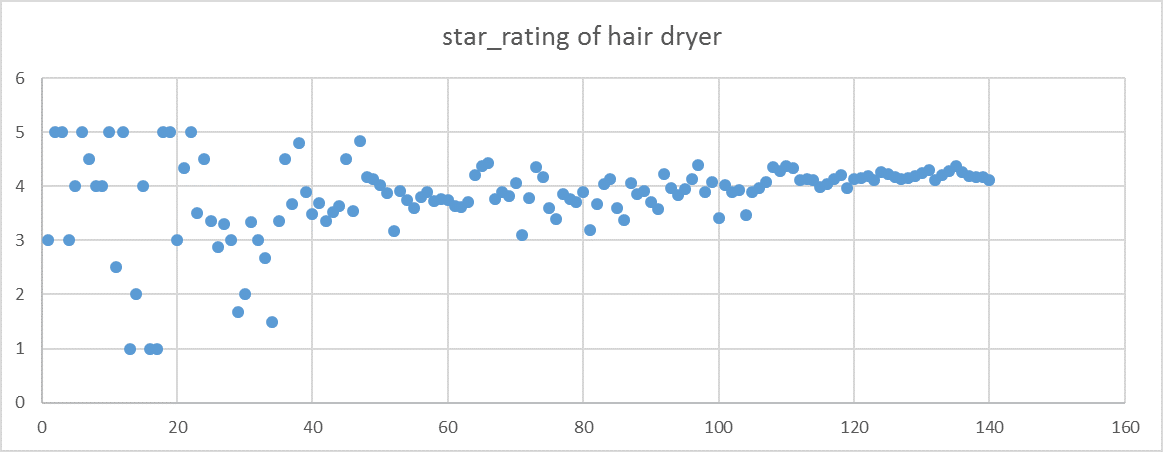
\includegraphics[width=.85\textwidth,height=3cm]{figures/a.png}
\caption{mean\_star\_rating for hair dryer}
\end{figure}

\item  Step 3 : Equation selection based on OLS

\quad \quad Use OLS (ordinary least squares) method to find the best fit. Least squares are very common, and its principle is relatively simple, so we omit it here. Here we use the results of microwave ovens as an example:
\end{itemize}

\begin{figure}[H]
\centering
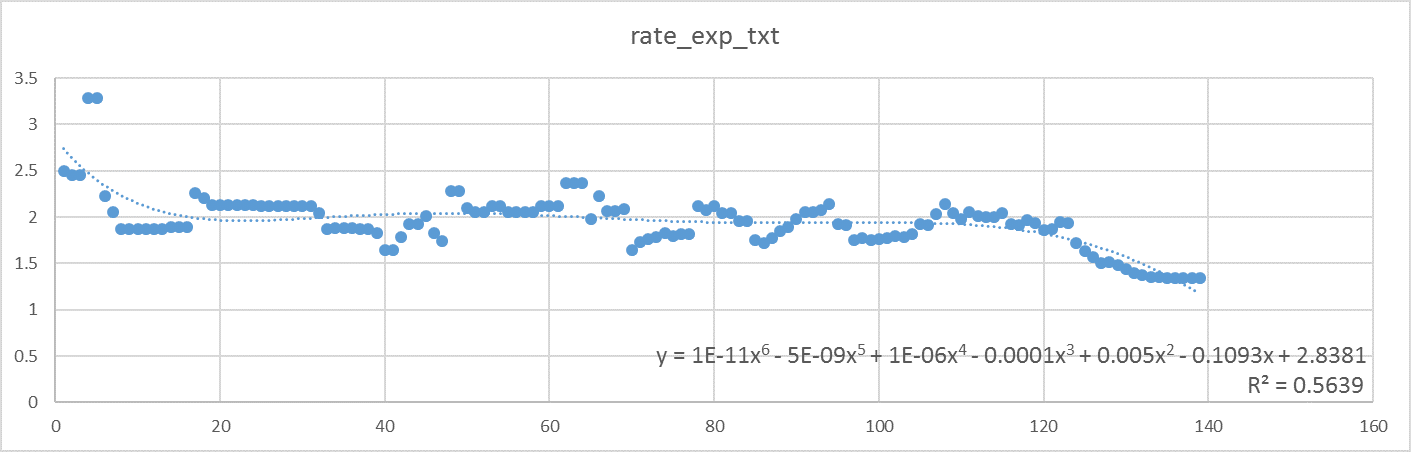
\includegraphics[width=.85\textwidth,height=3cm]{figures/b.png}
\caption{rate\_exp\_txt }
\end{figure}

\begin{figure}[H]
\centering
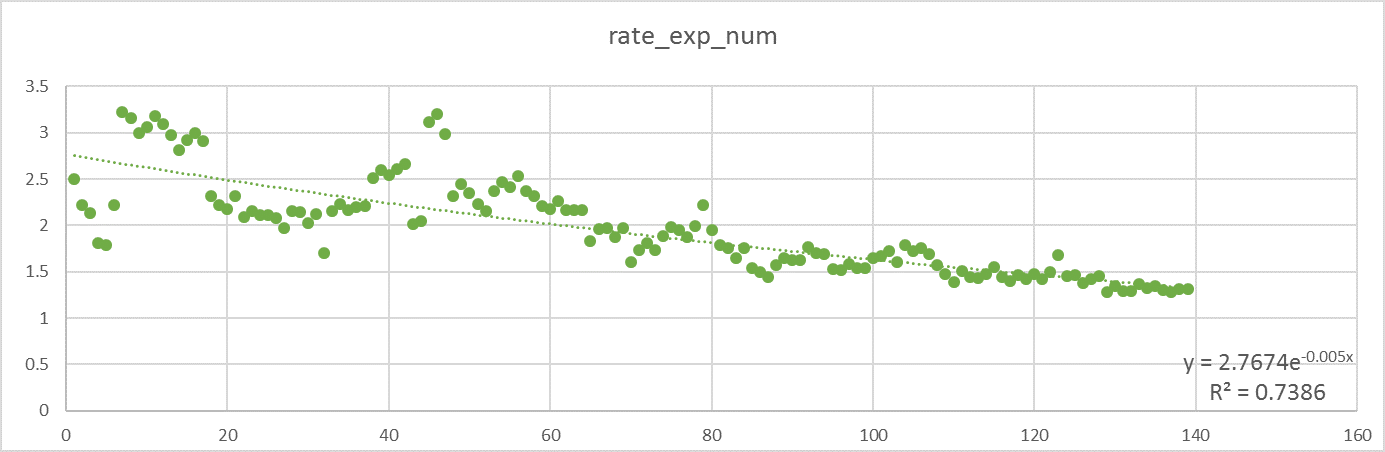
\includegraphics[width=.85\textwidth,height=3cm]{figures/c.png}
\caption{rate\_exp\_num }
\end{figure}

\begin{figure}[H]
\centering
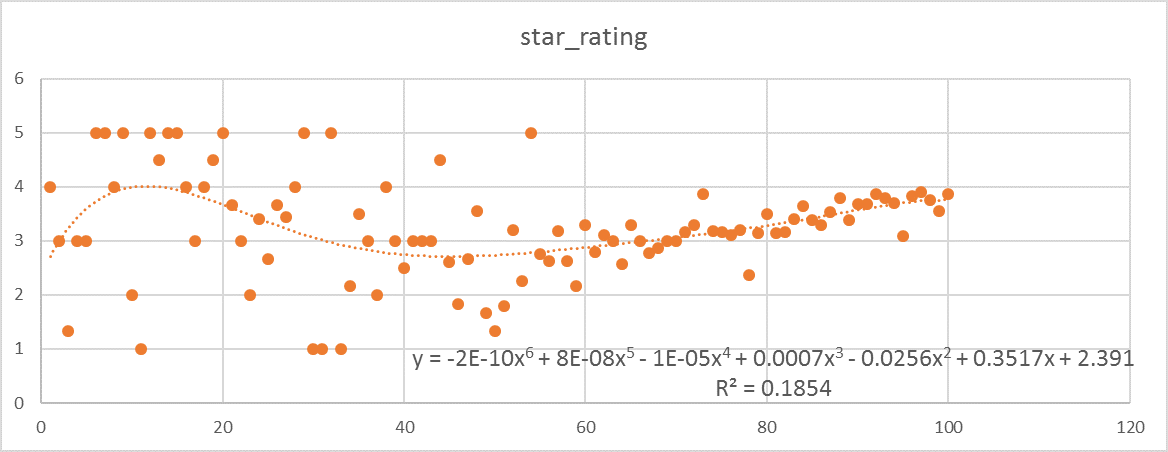
\includegraphics[width=.85\textwidth,height=3cm]{figures/d.png}
\caption{mean\_star\_rating}
\end{figure}

\begin{longtable}[c]{ccc}
\caption{Results of Reputation Fitting - MV}\\
\toprule
 & $R^2$ & Equation \\
\midrule
\endhead
\bottomrule
\endfoot
rate\_exp\_txt & 0.5639 & 
$y= −0.0001x^3+ 0.005x^2 -0.1093x+ 2.8381$ \\
rate\_exp\_num & 0.7386 & $y= 2.7674e^{−0.005x}$ \\
star\_rating & 0.1854 & $y=−0.0007x^3- 0.0256x^2+ 0.3517x+ 2.391$\\
\end{longtable}

The fitting effects of three measures are different. As shown in the table 4, the fitting effect of $star\_rating$ is the worst, which means that if it is used to represent reputation,  the trend over time will be difficult to detect, because it fluctuates much. From Figure 5-7, microwave ovens' reputation is on a downward trend according to $rate\_exp\_txt$ and $rate\_exp\_num$, however, according to star\_rating, the trend change is not obvious. Actually, for baby pacifiers and hair dryers, the situations are similar.

\subsection{Measure Combinations that Indicate Products' Success/ Failure}

\subsubsection{Aggregation Processing}

\quad \quad For different products, the factors that affect their success or failure are different. we aggregated the product types by $product\_parent$ and gathered data on a monthly basis as the time factor is also indispensable for the prediction of the factors causing the success or failure.

\subsubsection{Corner Detection}

\quad \quad We view the inflection point in the product sales time series as a sign of potential success or failure, because it means that the product is starting to turn, and the company should recognize this and remedy it before the product actually fails. Mann—Kenddall method is used to detect those inflection points, it is a non-parametric method, which means it does not need samples to follow a certain distribution, and is not disturbed by a few outliers. It is more suitable for sequential variables and easy to calculate:

For the time series $X$ with $n$ sample sizes, construct:
\begin{equation}
    S_k= \sum_{i=1}^kr_i, 
\end{equation}
\begin{equation}
    where \quad r_i=\left\{
\begin{array}{rcl}
1     &      & {x_i > x_j}\\
0     &      & else
\end{array} \right.        j=1,2,...,i 
\end{equation}

Under the assumption of random independence of time series:
\begin{equation}
     UF_k=\tfrac{S_k-E(S_k)}{\sqrt{Var(S_k)}} ,k=1,2,...,n 
\end{equation}

where $UF_1=0$, mean $E(S_k)=\tfrac{n(n+1)}{4}$, and variance $Var(S_k)=\tfrac{n(n-1)(2n+5)}{72}$

In the case of a product with $product\_parent$ is 732252283, the result of detecting the inflection point is as followed:

\begin{figure}[h]
\centering
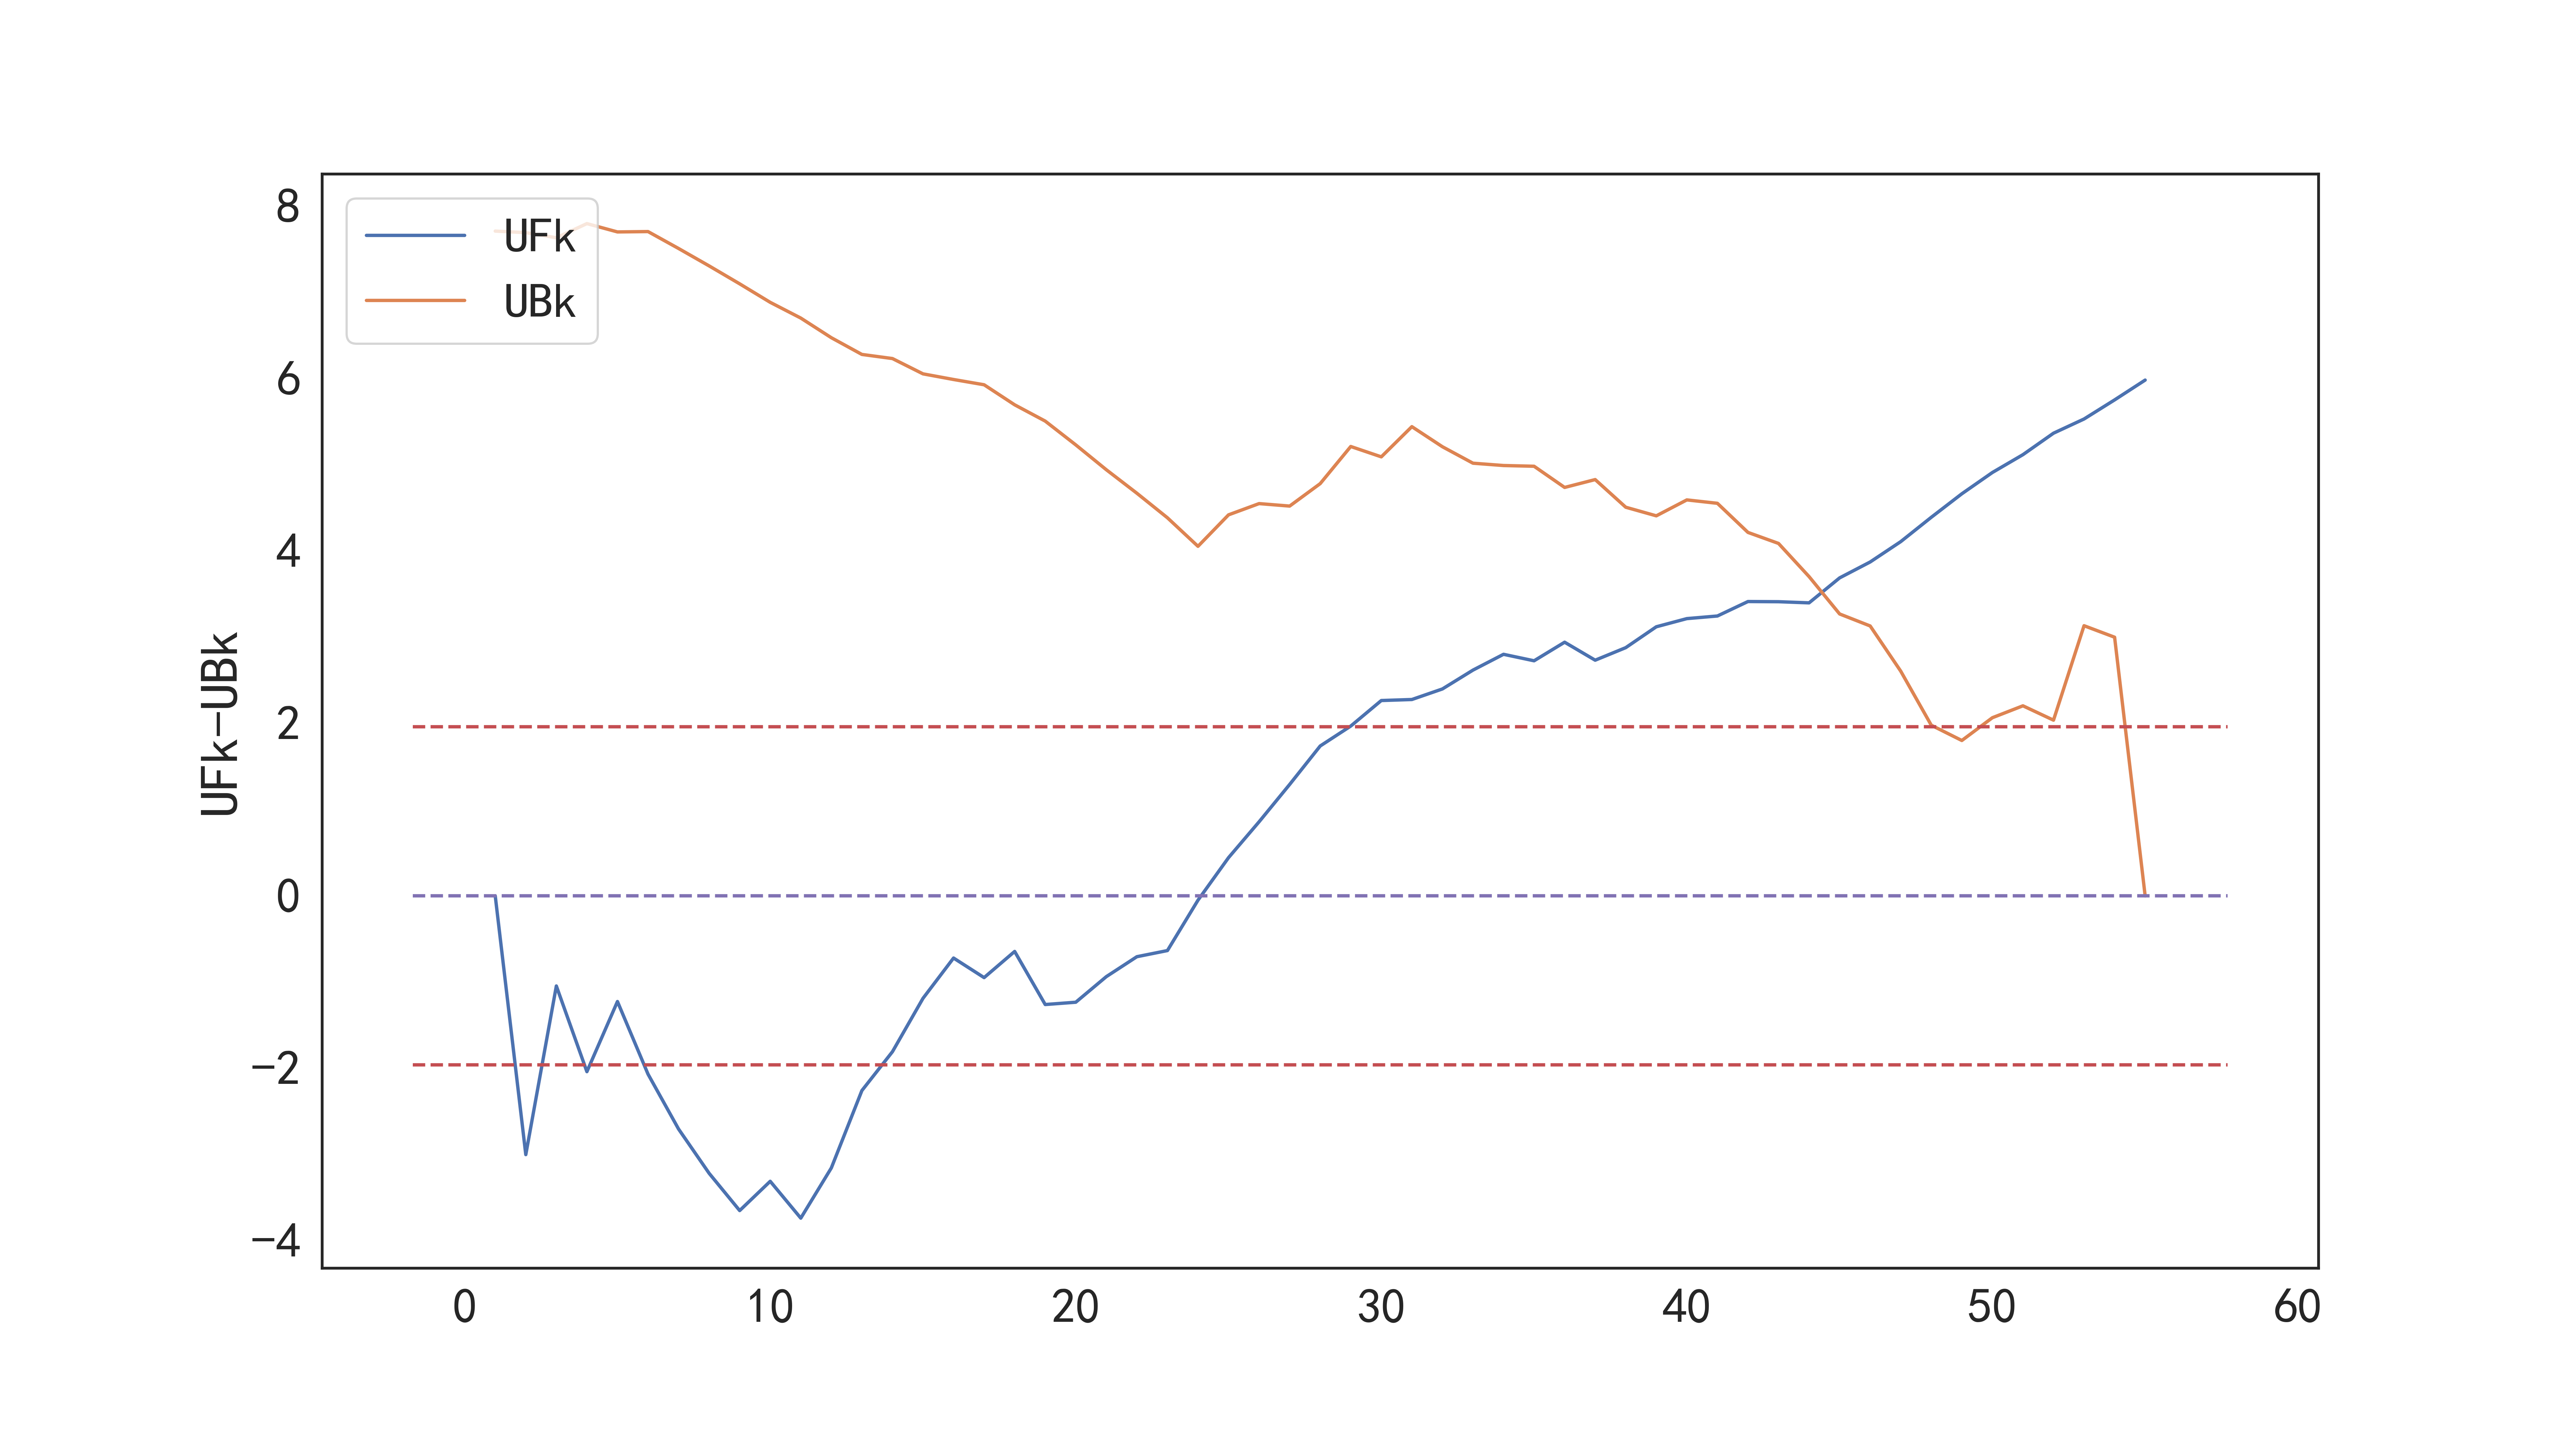
\includegraphics[width=.95\textwidth,height=6cm]{figures/k.png}
\caption{Results of Detection}
\end{figure}

As the UFK and UFK graphs show, when the value of UFK or UFK is greater than 0, the sequence shows an upward trend, while less than 0 indicates a downward trend. When they exceed the critical line, they indicate a significant upward or downward trend.The range beyond the critical line is defined as the time zone in which the inflection occurs. If two curves of UFk and UBk intersect and the intersection point is between the critical boundary, this point symbolizes the time when the inflection begins.

\subsubsection{Regression}

\quad \quad To determine the combinations of text-based and ratings-based measures that best indicate a potentially success or failure, we construct another linear regression based on the data of the year before the inflection point.

\begin{longtable}[c]{cccc}
\caption{Importance given by Regression Model}\\
\toprule
variabels  &  importance & variabels  & importance\\
\midrule
\endhead
\bottomrule
\endfoot
two\_sided     & 0.6430 & understandable        & 0.0339 \\
positive       & 0.1548 & star\_rating          & 0.0211 \\
complexity     & 0.0457 & att\_pos              & 0.0140 \\
negetive       & 0.0407 & star\_rating\_helpful & 0.0133 \\
\end{longtable}

\quad The results turned out the linear regression fits well, for 4.5820 for mean squared error and 0.9244 for $R^2$. From the result, the measure combinations that detect the potential success or failure of products are review's $two-sided$ attribute, $positive$ and $complexity$. 

\quad That means a product with more two-sided reviews and convey more positive, detailed information may lead to a success.

\subsection{Relationship Between Ratings and Review Types}

\subsubsection{Fluctuation Correlation Model}

\quad \quad We establish a model to test the fluctuation correlation between two groups of variables. Fluctuations are deviations from expected values. For each time series, extract out its fluctuation characteristics series(FCS)[14], then calculate the correlation between two FCS which indicates the sequence and causality between these two original series. The detailed fluctuation correlation modeling steps are as follows:
\newpage
\begin{itemize}
\item  Step 1 : Prediction method selection

\quad \quad Actually we have tried many prediction methods, and use mean-square error(MSE) as the optimization criterion, and finally, exponential smoothing method is determined to be the prediction method. Since the principle of exponential smoothing is very basic, here we omit it.

\item  Step 2 : Extraction of the FCS

\quad \quad The predicted series is subtracted from the original series to obtain FCS, as is shown in the figure below.
\begin{figure}[H]
\centering
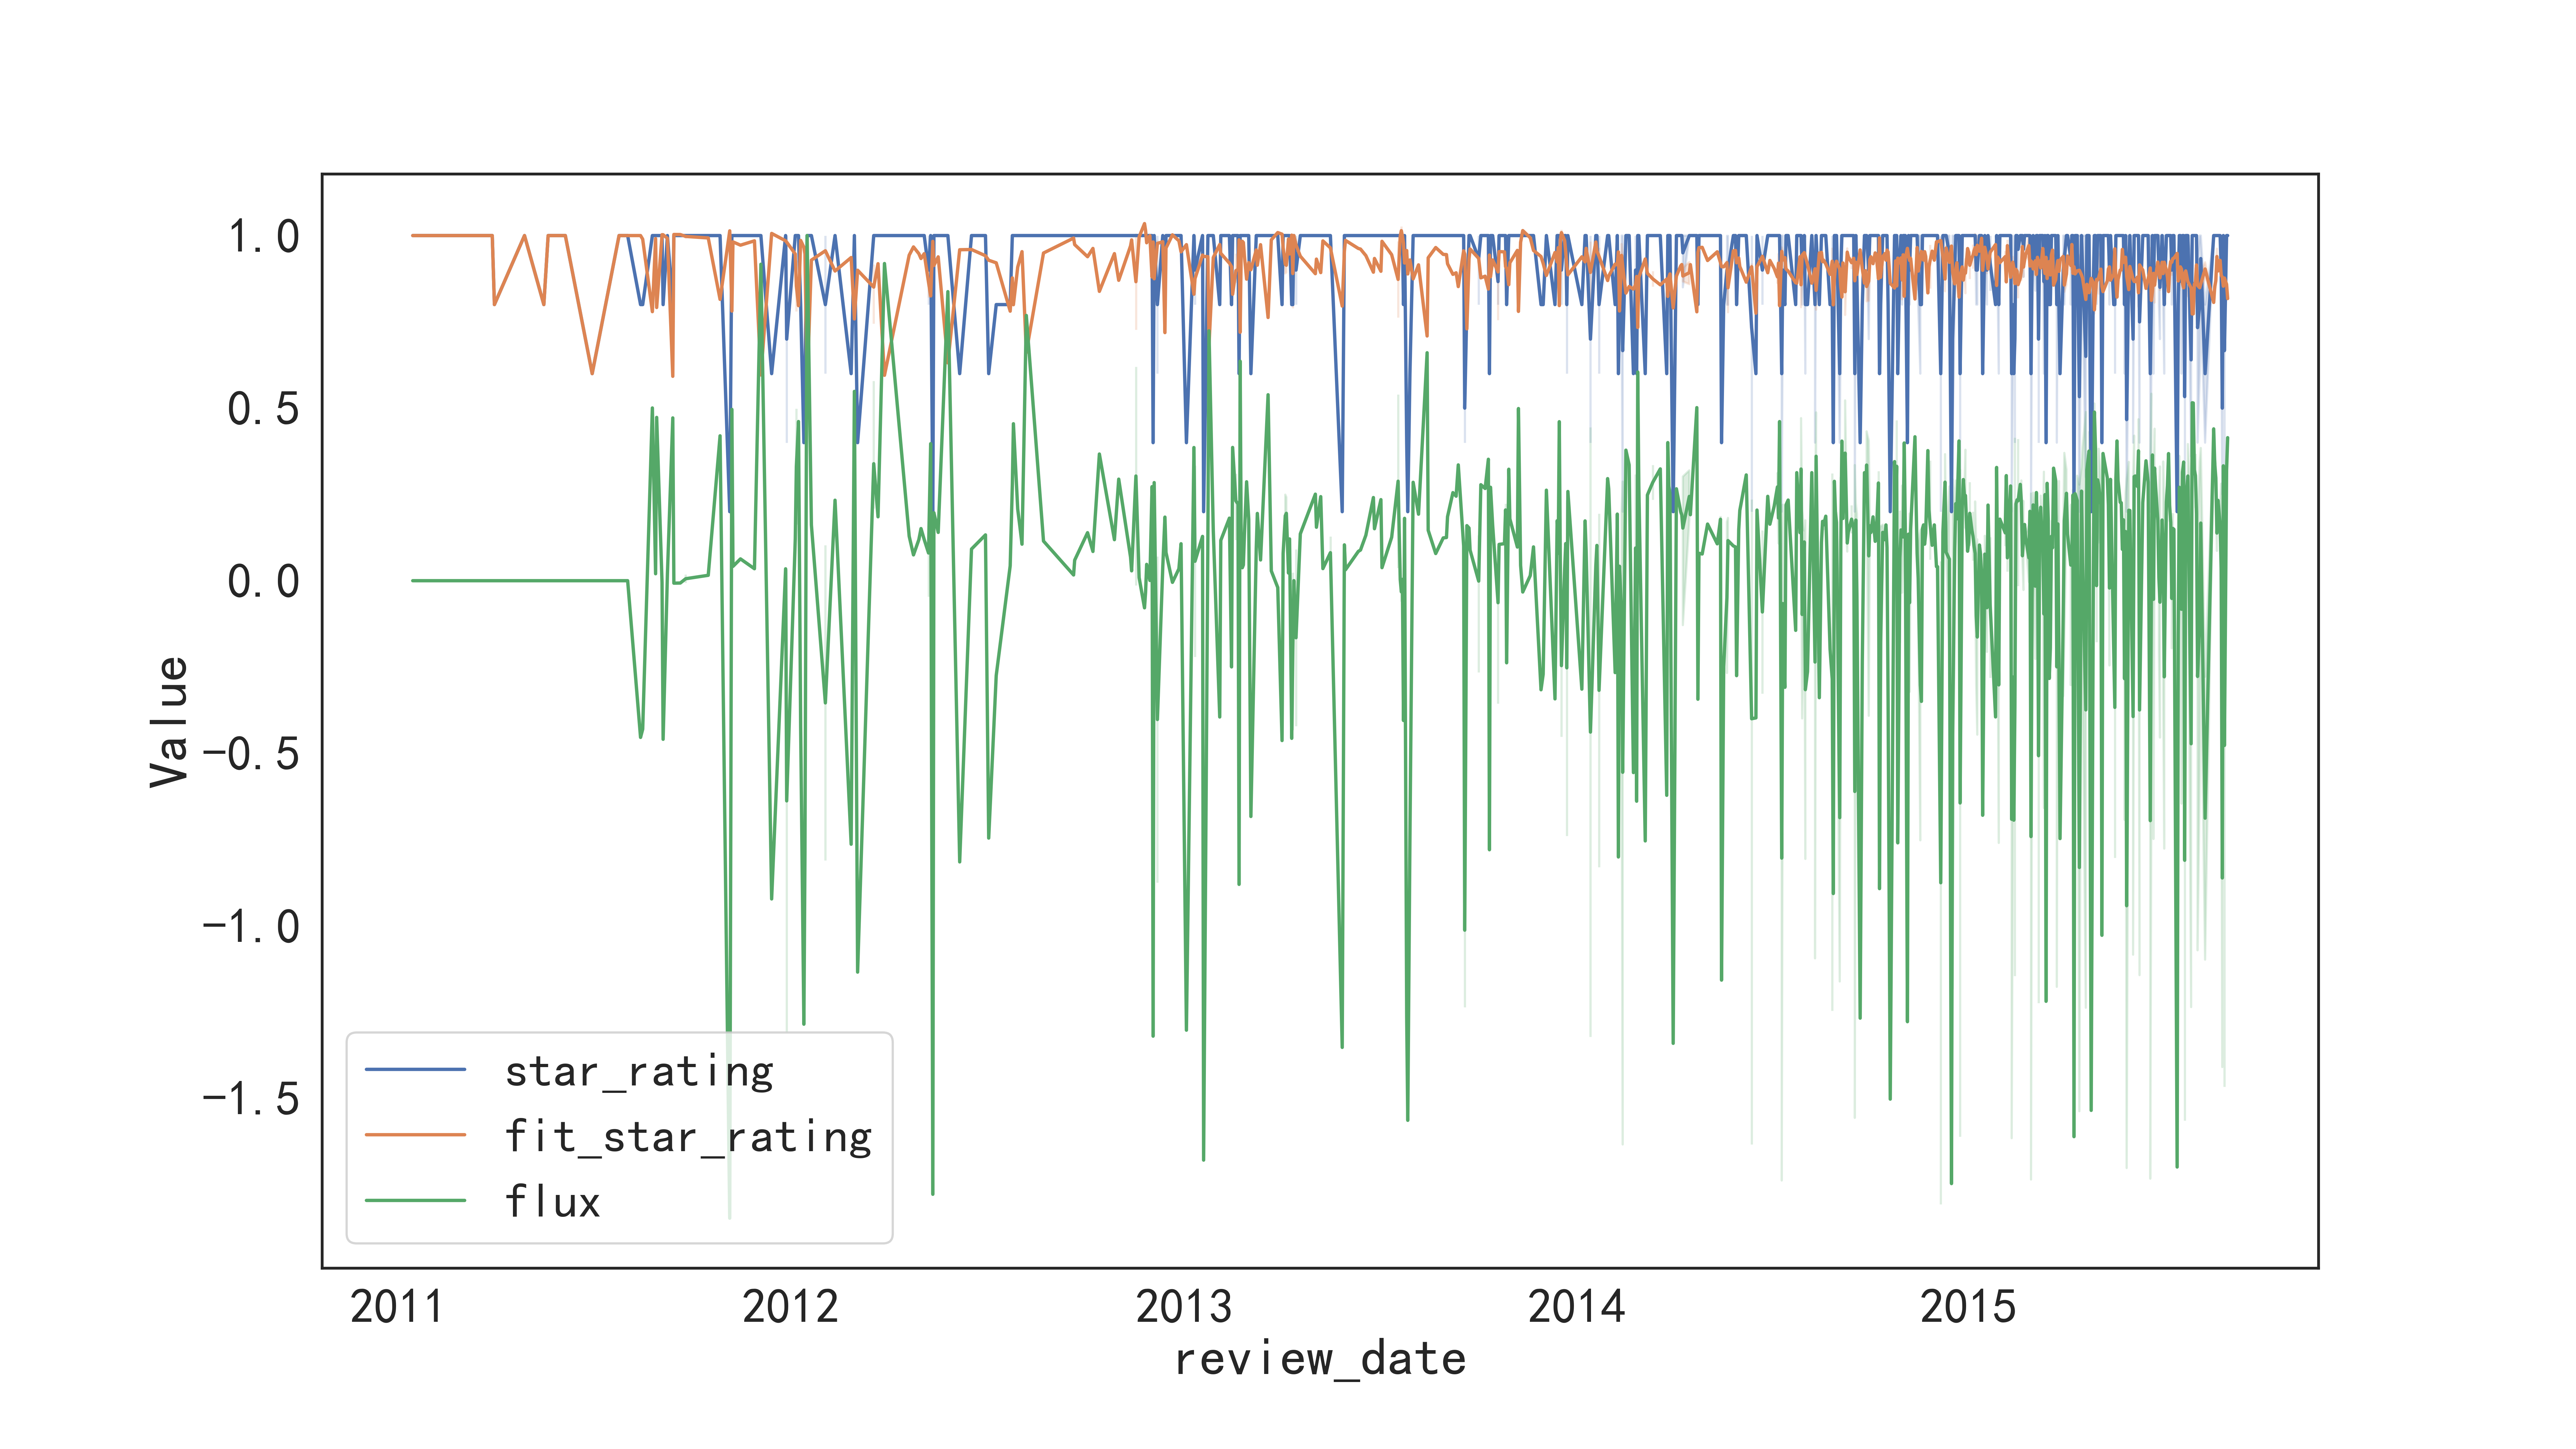
\includegraphics[width=.95\textwidth,height=5.5cm]{figures/f.png}
\caption{Step 2: Extraction of the FCS}
\end{figure}
\item  Step 3 : Correlation between FCS

\quad \quad To calculate the correlation between FCS, and to get the final fluctuation correlation between the original series. There are many alternative methods of correlation analysis, such as J-measure, pearson correlation, spearman correlation, Granger and so on.  

\end{itemize}

\subsubsection{Quantification of Review Types}

\quad \quad In Part \uppercase\expandafter{\romannumeral1}, we have obtained the attitude levels in part 4.2.2. Here we use $positive$,$negative$ and $neutral$ scores to symbolize the type of reviews. The larger the positive score is, the more positive the review.

\subsubsection{Correlation Analysis and Results}

\quad \quad Before correlation analysis, time series are shifted to judge whether start rating can cause the change of review types, since there is a certain time lag between when consumers see the star rating in the previous period and when they write down their own reviews. Here the series of positive scores is translated back one period (about one to sixty days according to the data). 

The correlation analysis include two parts: 
\begin{enumerate}[leftmargin=*,fullwidth,itemindent=2em,label=(\arabic*)]
\item{Common Correlation Analysis}

\quad \quad Analyze the correlation between the original time series of star\_rating and positive degree. As is shown in the table (df is the degree of freedom), all the data do not conform to the normal distribution. Therefore, spearman correlation analysis is adopted to calculate the correlation.

% Please add the following required packages to your document preamble:
% \usepackage{longtable}
% Note: It may be necessary to compile the document several times to get a multi-page table to line up properly
\begin{longtable}[c]{ccccccc}
\caption{Test results of normality}\\
\toprule
     & \multicolumn{3}{c}{Kolmogorov-Smirnova} & \multicolumn{3}{c}{Shapiro-Wilk} \\
\midrule
\endhead
\bottomrule
\endfoot
     & coefficient    & df    & significance   & coefficient & df  & significance \\ \hline
f1   & .255           & 833   & .000           & .768        & 833 & .000         \\
f2   & .073           & 833   & .000           & .967        & 833 & .000         \\
star & .437           & 833   & .000           & .543        & 833 & .000         \\
pos  & .152           & 833   & .000           & .867        & 833 & .000         \\
\end{longtable}

\quad \quad The result of spearman correlation analysis is 0.27, and P value = 0.000 < 0.01. So star rating and the positive degree of reviews are significantly positively correlated, while the degree of correlation is not high.

\item{Fluctuation Correlation Analysis}

\quad \quad Extract FCS of these two original series (f1 and f2), and analyze the fluctuation correlation between the original time series by calculating the correlation coefficients of the two FCS.

\quad \quad f1 and f2 also do not conform to the normal distribution, and the result of spearman correlation is 0.224, with P value < 0.01. Therefore, we can assume that high star ratings can incite more positive reviews.


\end{enumerate}


\subsection{Relationship Between Ratings and Review Descriptors}

\subsubsection{Quantification of Review Descriptors}

\quad \quad For each review descriptor, we give two quantitative measures. One is the simple counting, and the other is based on the sentiment extracted in part 4.2.2.

\subsubsection{Results}

\begin{longtable}{ccccc}
\caption{Distribution for 'great' of Hair Dryer}\\
\toprule
\makebox[0.16\textwidth][c]{star\_rating} &  
\makebox[0.16\textwidth][c]{positive} &
\makebox[0.16\textwidth][c]{neutral} & 
\makebox[0.16\textwidth][c]{negative} &
\makebox[0.16\textwidth][c]{total} \\
\midrule
\endhead
\bottomrule
\endfoot
5            & 344      & 1608    & 2        & 1954  \\
4            & 49       & 477     & 0        & 526   \\
3            & 0        & 130     & 0        & 130   \\
2            & 0        & 79      & 0        & 79    \\
1            & 0        & 82      & 0        & 82    \\ 
\end{longtable}

\quad \quad As shown in the table 5, the descriptor 'great' is generally strongly associated with rating levels, and the higher the level, the more it appears. However, according to our sentiment measure, although 'great' appears in 5 star review, it doesn't necessarily mean this review is positive. But the conclusions vary from different descriptors, as is shown in appendix.


\section{Part \uppercase\expandafter{\romannumeral3}: Feature extraction of specific products}

\quad \quad By using TF-IDF toghther with Spectral Co-Clustering algorithm described before, we can easily extract some best words by normalized cuts and comparing sums inside and outside the bicluster.

The extracted topic words can help with the analysis with the advantage and disadvantages about a product by combining the relationship between the contents of those keywords and the product's $star\_rating$, including adjusted rating meatures by $num$ and $txt$ methods. Here are some of the keywords we extracted  and we made them into several word clouds for a clearer presentation. You can view more example clouds in Appendix.
\begin{figure}[H] 
\centering
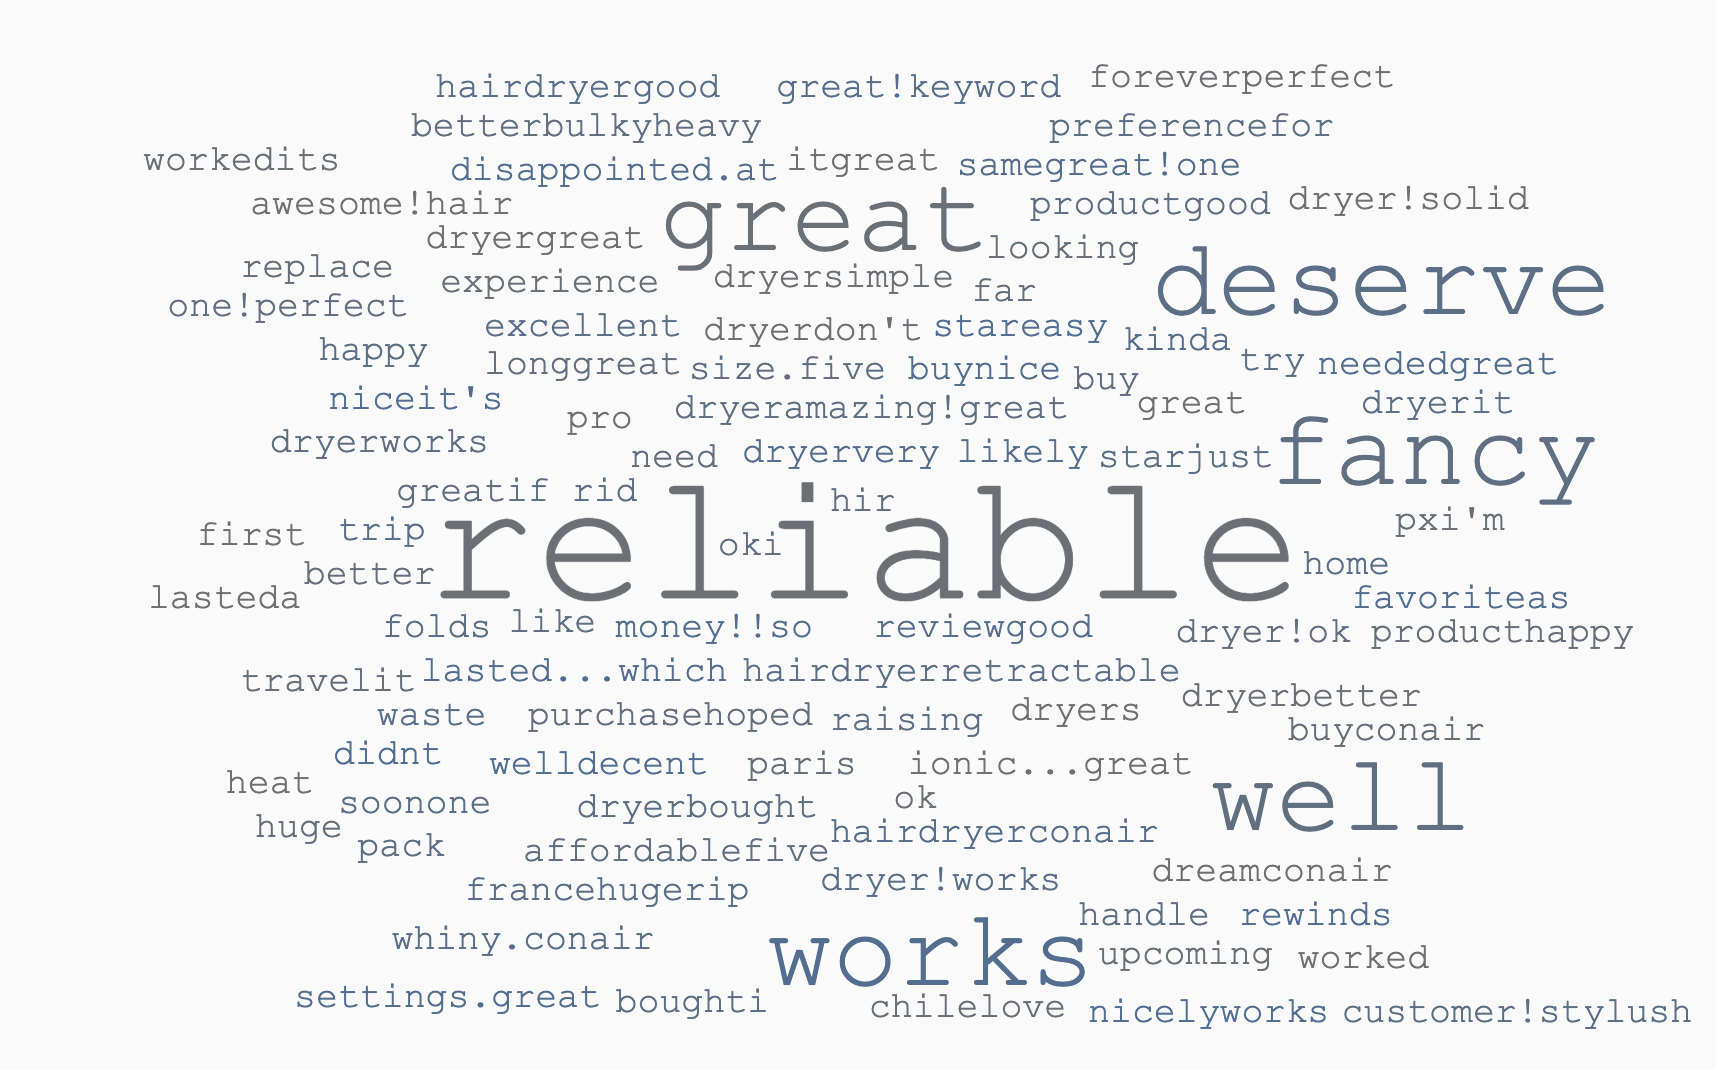
\includegraphics[width=.9\textwidth,height= 7.5 cm]{figures/cloud.png}
\caption{Key reviews of hair dryer 423960}
\end{figure}

\section{Model Evaluation}

\subsection{Review Helpfulness Model}

\quad \quad When using two or more methods to do evaluation, the consistency  between the two evaluation methods' results should be tested, so it is necessary to carry out the correlation test for the two results in part 4.3.3. 
The normality test results of review helpfulness scores shows that, both of the results do not conform to the normal distribution. Therefore, spearman and kendall correlation analysis are adopted. Through calculation, the result is:

\begin{longtable}[c]{ccccc}
\caption{Results of correlation analysis}\\
\toprule
                                                            & \multicolumn{2}{c}{Spearman} & \multicolumn{2}{c}{Kendall} \\
\endhead
\bottomrule
\endfoot
                                                            & coefficient  & significance  & coefficient  & significance \\ \hline
\begin{tabular}[c]{@{}c@{}}EWM \\ v.s.\\  TOPSIS\end{tabular} & .974         & .000          & .916         & .000         \\
\end{longtable}

\subsection{Regression Model}
\quad \quad After several regression model, one thing that really matters is to do some diagnosis plots to see whether the model is well-fitted. Here we presents a example of hair dryer to illustrate the accuracy of our model.
\begin{figure}[H] 
\centering
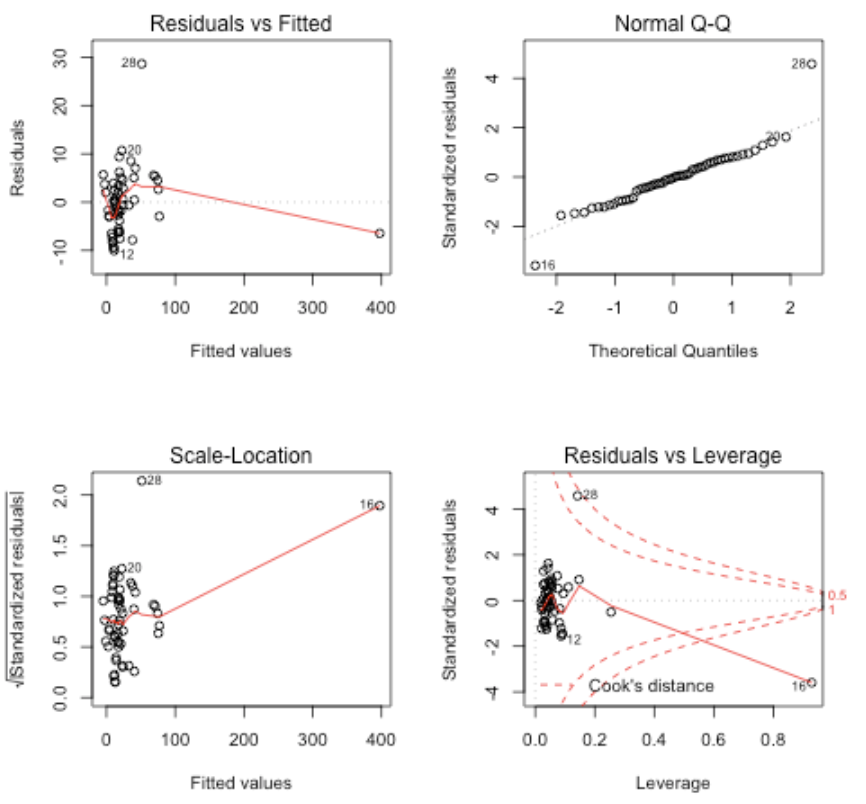
\includegraphics[width=.9\textwidth,height=8cm]{figures/qq.png}
\caption{Regression diagnosis}
\end{figure}
\quad These two sets of figures show that the polynomial regression fitting effect is ideal, and basically meets the linear assumption, residual normality test, and homoscedasticity. You can view more diagnosis plots in Appedix of other products.

\section{Strengths and weaknesses}

\subsection{Strengths}
\begin{itemize}
\item \textbf{Substantial and Detailed}\\
Our research content is very rich, on the basis of deeply mining data sets and composing new measures, we also build more than three models to do analysis, and get a lot of considerable conclusions.
\item \textbf{Solid theoretical support}\\
All of our methods and models are supported by academic literature with available sources.
\end{itemize}

\subsection{Weaknesses}
\quad \quad Due to the limited content of the datasets, when building the review helpful evaluation model, the amount of indexes is far from enough. Therefore, the helpfulness score may be underestimated compared with the reality.

\begin{thebibliography}{99}
\bibitem{1} Jia-Lang Seng, T.C. Chen, An analytic approach to select data mining for business decision, Expert Systems with Applications,
Vol 37, pp. 8042-8057, 2010.
\bibitem{2} U. Fayyad, G. Piatetsky-Shapiro, P. Smyth, From data mining to knowledge discovery in databases, AI Magazine (1996), pp. 37–53.
\bibitem{3} Indranil Bose, Radha K. Mahapatra,
Business data mining — a machine learning perspective, Information and Management, Vol 39, 2001, pp. 211-225,
\bibitem{4} Shankhadeep Banerjee, Samadrita Bhattacharyya, Indranil Bose, Whose online reviews to trust? Understanding reviewer trustworthiness and its impact on business, Decision Support Systems, Vol 96, 2017, pp. 17-26,
\bibitem{5} Zhou, S. S. and Guo, B. The order effect on online review helpfulness: A social influence perspective. Decision Support Systems 93, 2017, pp. 77-87. 
\bibitem{6} Hai, Z., et al. A statistical nlp approach for feature and sentiment identification from chinese reviews. in CIPS-SIGHAN Joint Conference on Chinese Language Processing. 2010.
\bibitem{7} Ghorpade, T. and L. Ragha. Featured based sentiment classification for hotel reviews using NLP and Bayesian classification. 2012 International Conference on Communication, Information and Computing Technology. 2012.
\bibitem{8} Flank, S. A layered approach to NLP-based information retrieval. 17th International Conference on Computational Linguistics, Volume 1. 1998.
\bibitem{9} Li, H. and Z. Lu. Deep learning for information retrieval. in Proceedings of the 39th International ACM SIGIR conference on Research and Development in Information Retrieval. 2016.
\bibitem{10} Smeaton, A.F., Using NLP or NLP resources for information retrieval tasks, in Natural language information retrieval. 1999, Springer. p. 99-111
\bibitem{11}  Li, S. An overview of Legibility Research J. Journal of PLA Foreign Language Institute, 20004:1-5.
\bibitem{12} Chen, M.-Y.J.O.I.R., Can two-sided messages increase the helpfulness of online reviews? 2016.
\bibitem{13} Zhao, F. An analysis of the usefulness of online customer reviews in Amazon. com. 2018, Guangdong University of Foreign Studies
\bibitem{14} Su, Y., et al. CoFlux: robustly correlating KPIs by fluctuations for service troubleshooting. in Proceedings of the International Symposium on Quality of Service. 2019.

\end{thebibliography}

\clearpage
\begin{appendices}
\section*{Appendix A}
\begin{longtable}{ccccc}
\caption{Distribution for 'problem' and 'problems' of Microwave Ovens}\\
\toprule
\makebox[0.16\textwidth][c]{star\_rating} &  
\makebox[0.16\textwidth][c]{positive} &
\makebox[0.16\textwidth][c]{neutral} & 
\makebox[0.16\textwidth][c]{negative} &
\makebox[0.16\textwidth][c]{total} \\
\midrule
\endhead
\bottomrule
\endfoot
5   & 0        & 56      & 0        & 56    \\
4   & 0        & 31      & 0        & 31    \\
3   & 0        & 16      & 0        & 16    \\
2   & 0        & 20      & 0        & 20    \\
1   & 0        & 99      & 0        & 99    \\ 
\end{longtable}

\begin{longtable}{ccccc}
\caption{Distribution for 'bad' of pacifiers}\\
\toprule
\makebox[0.16\textwidth][c]{star\_rating} &  
\makebox[0.16\textwidth][c]{positive} &
\makebox[0.16\textwidth][c]{neutral} & 
\makebox[0.16\textwidth][c]{negative} &
\makebox[0.16\textwidth][c]{total} \\
\midrule
\endhead
\bottomrule
\endfoot
5     & 3     & 98      & 0      & 101      \\
4       & 1      & 48      & 0      & 49      \\
3     & 0     & 30       & 0   & 30    \\
2    & 0      & 26    & 0    & 22   \\
1  & 0    & 22    & 2    & 28  \\
\end{longtable}
\section*{Appendix B}
\begin{figure}[H] 
\centering
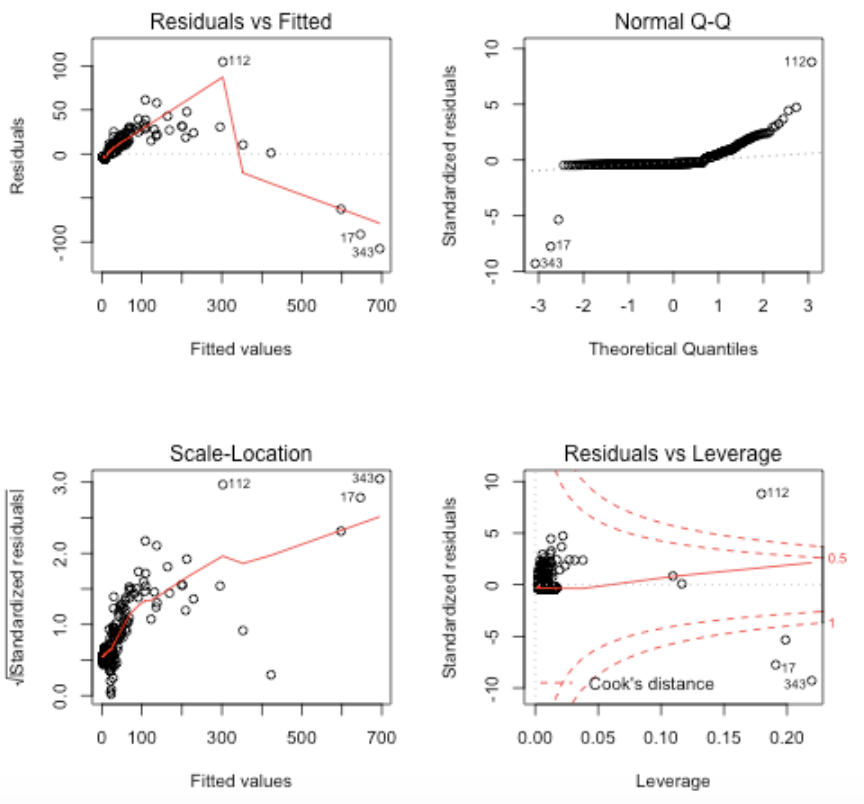
\includegraphics[width=.9\textwidth,height=8.5cm]{figures/qq2.png}
\caption{Regression diagnosis}
\end{figure}

\begin{figure}[H] 
\centering
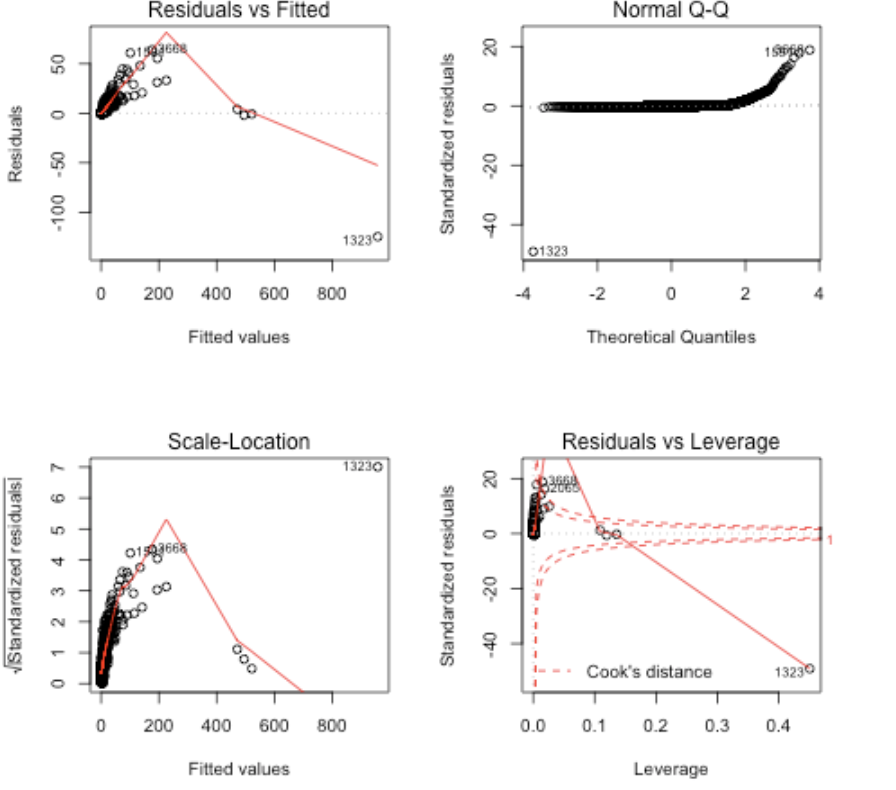
\includegraphics[width=.9\textwidth,height=8.5cm]{figures/qq3.png}
\caption{Regression diagnosis}
\end{figure}
\section*{Appendix C}
\begin{figure}[H] 
\centering
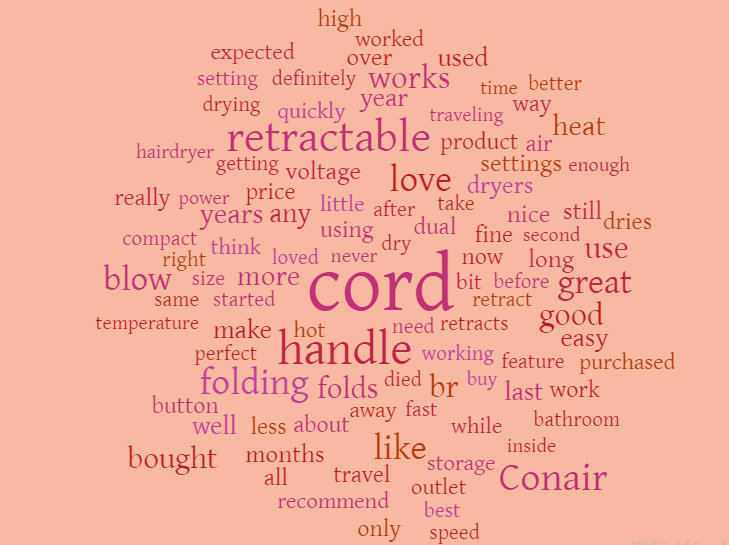
\includegraphics[width=.9\textwidth,height=5.5cm]{figures/yun1.png}
\caption{Key reviews of hair dryer 423960}
\end{figure}

\begin{figure}[H] 
\centering
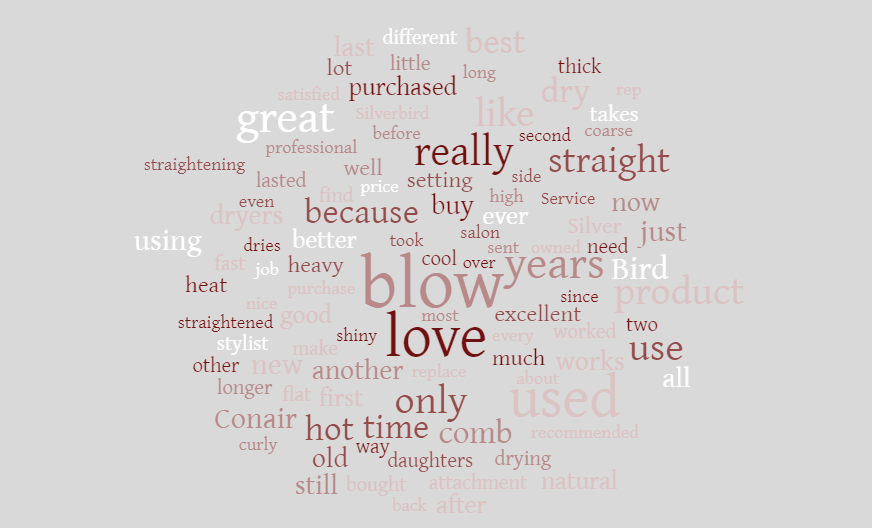
\includegraphics[width=.9\textwidth,height=5.5cm]{figures/yun2.png}
\caption{Key reviews of hair dryer 423960}
\end{figure}

\begin{figure}[H] 
\centering
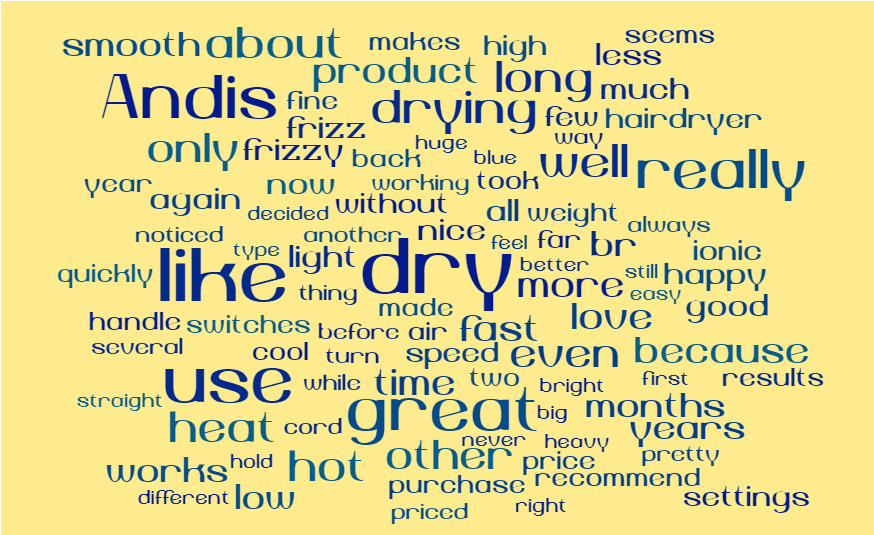
\includegraphics[width=.9\textwidth,height=6cm]{figures/yun3.png}
\caption{Key reviews of hair dryer 423960}
\end{figure}



%Here are simulation programmes we used in our model as follow.\\

%some more text\\

%\textcolor[rgb]{0.98,0.00,0.00}{\textbf{Input Python source:}}
%\lstinputlisting[language=Python]{./code/Housing.py}
\end{appendices}
\end{document}
